\chapter{Group Anomaly as Basis for Protest Detection}
\label{ch:absenteeism}
%\chapter{Event Detection based on Information Absenteeism}
%Information Absenteeism Detection on Social Graphs
% if you want to define paper specific  macros
% then put everthing between begingroup and endgroup
\begingroup
\newcommand{\score}{S}
\newcommand{\myalgo}{CoolAlgo}


%\begin{abstract}
%Event detection in online social media has primarily focused on identifying
%abnormal spikes, or bursts, in activity. However, disruptive events such as socio-economic disasters, civil unrest, and even power outages, often result in abnormal troughs involving group absenteeism of activity. We present the first study, to our knowledge, that models absenteeism and uses detected absenteeism as a basis for event detection in location based social networks (LBSN) such as Twitter. Our framework addresses the challenges of (i) early detection of absenteeism, (ii) identifying the point of origin, and (iii) identifying groups or communities underlying the absenteeism. Our approach uses the formalism of graph wavelets to represent the spatiotemporal structure and user activity in a LSBN. This formalism affords multiscale analysis, enabling us to detect anomalous behavior at different graph resolutions, which in turn allows identification of event location and anomalous groups underlying the network. We introduce a systematic two-pass detection method using graph wavelets to detect group absenteeism and then check if there is a subsequent activity spike. The effectiveness of our approach is highlighted with three case studies involving Twitter activity over Latin American countries.
%\end{abstract}


% mainfile: ../main.tex
\section{Introduction}
This chapter was published in the 20th ACM SIGKDD international
conference on Knowledge discovery and data mining (KDD 2014)~\cite{jin2014misinformation}.

In recent years social networking sites such as Twitter and Facebook have
provided not just a platform for communication but also a means
of mobilization and strategic interaction between key players
of social movements, e.g., protests. Traditionally social movements occur
within a subset of the population and have spread through on-the-ground
communities and unions. With the advent of leaner communication
technologies like Twitter, the way such movements form and
spread through modern society has changed. With Twitter, in particular,
traditional slogans have transformed into hashtags which can
offer a consistent way of communicating the reason and
motivation of social movements like protests and uprisings.

\begin{figure}[h]
\centering
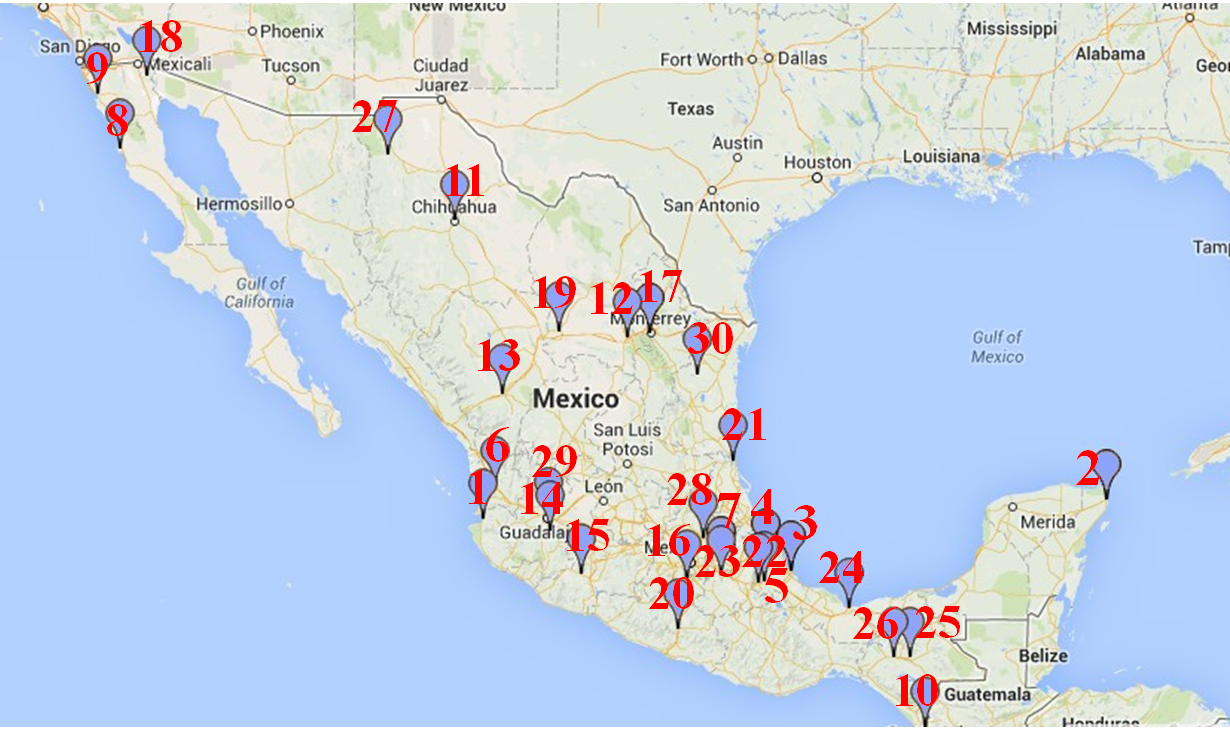
\includegraphics[scale=0.4]{figures/mexico_teacher_protest.png}
\caption{Mexico teacher protest events from Sep 1 to Sep 7, 2013. The blue pins denote protest cities; the numbers in red denote the sequence of
protests as they spread across the country.}
\label{fig:mexico_teacher}
\end{figure}


In this chapter, we focus on Twitter's
user networks during protests
and similar civil unrest activities in Latin America. Our goals
are to model the propagation and growth of contagion-like protest
waves within a social network and to understand the social and
structural dynamics underlying such phenomena. The key problem
is understanding the nature of information propagation among motivated
users of a social network. We have observed that such mass
protests emerge very swiftly and sharply. In Twitterspeak, they
would be considered trending but most such trends quickly decline
on the social network even if not in the physical world. Modeling
protest-related topic propagation on networks involves several challenges.

First, social protest propagation through online media can spread
over large areas more quickly than traditional
methods since users are geographically distributed. For example,
on September 1, 2013, the Mexican government's education reform bill drew
the wrath of teachers country-wide who opposed the reform
(which required regular assessments of their performance as educators).
Twitter was a virtual loudspeaker, providing a platform for organization
and strategization for teachers to put forth their arguments against
the bill. A series of mass teacher protests erupted and spread
from city to city. As shown in Fig.~\ref{fig:mexico_teacher}, we
see the movement spreading over time to different locations with
no obvious visual mobilization pattern. The second challenge is
that Twitter's user network embodies many subgraphs based on
social ties which might afford different propagation rates due to
subgraph-specific structures.

Thus identifying how the cause of a protest is adopted by Twitter users and how mobilization happens in the underlying network is a difficult task.
To address this problem we present an integrated framework with new
theoretical models as well as empirical validation on real Twitter
data for actual protests witnessed in the recent past. Our key
contributions are:

\iffalse
We also focus on the role of community driven information propagation over this bispace. We use \textit{Geometric Brownian Motion} (GBM) and Poisson processes over the mentions network and latent space respectively to model information propagation during mass social movements. When the protest-related information propagation starts, it propagates over the two spaces independently and simultaneously. In the mention network space, the propagation process follows Geometric Brownian diffusion over the defined social network. In the latent space, we believe propagation will obey the Poisson distribution. We introduce a trust function $S_t$ and Brownian distance $d_{ij}$ between users to describe the information propagation mechanism of the mentions network. Suppose that some user $v_i$'s trust with user $v_j$ at time $t$ is $S^{ij}_t$ and the distance from user $v_i$ to user $v_j$ is $d_{ij}$. Only when $ln(S^{ij}_t)$ is no less than the distance $d_{ij}$ is $v_j$ infected by $v_i$.
%We propose that the trust function $S_t$ follows a dynamic geometric Brownian motion
%\begin{equation}\frac{\partial S_t}{S_t} = \mu {dt}+\sigma dW_t
%\end{equation}


In the latent space, we model the propagation as a Poisson distribution, believing that it is difficult to account for all the ways in which information may spread. For a given time interval $T_p$, the probability of infecting users is expressed as $Pr(x=k)=\frac{\lambda^k e^{-\lambda}}{k!}$ where $\lambda$ is the average number of infected users during that time interval $T_p$.
\vspace{2 mm}
\fi

\begin{itemize}
\item
We model the inherent heterogeneity in propagation using a
bispace model, comprised of the Twitter mentions network (where
both globally and locally influential neighbors contribute to a user's
recruitment) and a
latent space (where external exposure to protest-related information is
captured).
\item We focus on the role of community-driven information propagation
over the bispace model. We use geometric Brownian motion (GBM)
over the mentions network and Poisson processes over the latent space to model information propagation during mass social movements.
\item We illustrate the effectiveness of our approach in modeling several key mass protest adoption scenarios in multiple countries of Latin America, viz.
Argentina, Brazil,
Colombia,
Mexico,
Uruguay, and
Venezuela.

\end{itemize}

The rest of this chapter is organized as follows. Section 2 covers related work in the areas of social movements, information diffusion in networks, external influences, and Brownian motion. Section 3 proposes the geometric Brownian motion propagation mechanism. Section 4 introduces the bispace propagation model, especially the model of propagation in latent space. In Section 5, we
present our dataset and experimental setup,
followed by initial experimental findings. Section 6 discusses the
evaluation results for our approach followed by a brief discussion in
Section 7.


%\section{Related Work}
We briefly review related work next, which comes from multiple areas.

\par \noindent
{\bf Social movements:}
Oliver and Myers~\cite{oliver1998diffusion}
develop a foundation for theoretical insights of social movements and
describe the limitations of simplified models. The Arab Spring of  2010
served as a context for many
researchers~\cite{gonzalez2011dynamics, bond201261, tufekci2012social, conover2013digital, saad2013mass}
to study the role
social networking sites play in the spread and recruitment
of participants in protests.
A detailed anatomy of
modern social protests is described by Saad-Filho~\cite{saad2013mass}
with the June 2013 anti-government protests in Brazil as a context.
In this work, we study the processes and sociological impacts of protests
in the modern era, fortified by online social networks and the
communities in and around them.\\

\vspace{-0.1in}
\noindent
{\bf Information diffusion in networks:}
Previous studies have approached the modeling of information propagation and
diffusion in social networks through several means, e.g.,
contagion models (SIR~\cite{castellini2007propagation}\, SISa~\cite{hill2010emotions}), diffusion based threshold and cascade models~\cite{kempe2003maximizing}, rise-and-fall patterns~\cite{matsubara2012rise}, coverage models~\cite{singer2012win}, and survival theory~\cite{rodriguez2013modeling}. A good survey of
different models of information diffusion is presented in~\cite{guille2013information}.\\

\vspace{-0.1in}
\noindent
{\bf External influences:}
We believe that the effects of influences that originate external
to the observed diffusion network, such as mass media
and offline spread of information, can impact the way in which information
flows within the online network.
Myers et al.~\cite{myers2012information} study the emergence of URLs
on Twitter with a probabilistic generative process using both
internal and external exposure curves in a contagion-like model.
Similar attention to the role of external factors is
paid by Crane and Sornette~\cite{crane2008robust} for
tracking the popularity of YouTube videos using a diffusion model.
Iwata et al.~\cite{iwata2013discovering} use
a shared cascade Poisson process model to discover
latent influences in social activities such as item adoption.
Using shared parameters among multiple Poisson processes, they were able to simulate sequences of item adoption events. \\

\vspace{-0.1in}
\noindent
{\bf Brownian motion:}
Zhou and colleagues (e.g.,~\cite{zhou2003distance, zhou2003network,
zhou2004network}) develop the notion of Brownian motion on networks
which they
use to discover communities of hierarchical structure both locally
and globally. We extend this approach in this chapter
to formulate a propagation algorithm based on geometric Brownian
motion (GBM). Borrowed from statistical physics, GBM has been
used heavily in finance to model stock price movements.
Scale invariance and the ability to model abrupt bumps
along propagation paths are the primary motivations for using GBMs
to model stochastic processes~\cite{tankov2004financial}. \\

\vspace{-0.1in}
\noindent
Our work builds on the concepts
introduced in~\cite{zhou2003network, iwata2013discovering, zhou2003distance, zhou2004network} but differs from the other diffusion models
described earlier by considering both the role of communities of
users and the abrupt nature of propagation of volatile information such as mass social protests. We include the notion of bispace where both latent (attributed to external influences) and observed user network influences are considered. We infer propagation rates for communities in the observed network and allow
implicit recruitment of users into protest actions through a Poisson process.


\section{Preliminaries} \label{sec:preliminaries}
In this section, we formalize our approach to event detection.
We first describe the accompanying notations in section~\ref{sec:notations} which will be used throughout the chapter.
Then we formally present our research problem statement, provide a brief comparison of our approach to a conventional solution, and review the challenging issues that are relevant to an event detection problem.
\subsection{Notations}
\label{sec:notations}
Let's assume we are given an undirected, weighted graph $\mathbf{G}(V,E,W;f)$, where $V=\{v_0,v_1,...,v_{N-1}\}$ represents the set of $N$ cities, $E$ refers to the connections between neighboring cities, and $W$ is a vector of non-negative weights associated with each edge $e_{ij}\in E$ as a function of geographical distance between a pair of vertices $(v_{i}, v_{j})$. The function, $f: V \rightarrow {\mathbb{R}}^N$ maps the vertices of graph $\mathbf{G}$, and $f(n)$ stands for the value on the vertex $v_n$. Graph $\mathbf{G}$'s adjacency matrix $\mathbf{A}$ is of size $N\times N$, where each element $a_{ij}$ is represented as:
\begin{equation}
a_{ij} = \left\{ \begin{array}{rl}
 w_{ij} &\mbox{ when $e_{ij}\in {E}$} \\
  0 &\mbox{ otherwise}
       \end{array} \right.
\end{equation}
Here, $\mathbf{A}$ is symmetric since $a_{ij}=a_{ji}$.
Let $d_i=\sum\limits_{v_j \in V}a_{ij}$ be the sum of all edge weights that are incident on $v_i$ and $\mathbf{D}$ be the diagonal matrix denoted as $\mathbf{D}=diag\{d_1,d_2,\ldots,d_N\}$. A Laplacian matrix $\mathcal{L}$ is defined as $\mathcal{L}=\mathbf{D-A}$. It is a symmetric matrix and has real eigenvalues $\lambda_{i}$ such that $0 = \lambda_{0} < \lambda_{1} \leq \lambda_{2} \leq \ldots \leq \lambda_{N-1} = \lambda_{max}$ and a complete set of $\mathcal{L}$'s normalized eigenvectors~\cite{bapat2010graphs} $\chi_{i}$ for $i=0,1,2,...,N-1$ described by:
\begin{equation}
\label{eq:eigenvalues}
\mathcal{L}\chi_{i}=\lambda_{i}\chi_{i}
\end{equation}
Obviously, $\chi_o(n)=\frac{\vec{\textbf{1}}}{\sqrt{N}}=\frac{1}{\sqrt{N}}\{1,1,...,1\}$, and is called direction component of $\mathbf{G}$.

\vspace{-1mm}
\paragraph{\textbf{Absenteeism Score}}
Although the raw volume of user interactions is a good indicator of users' online activities, it can be noisy and often exhibits a strong temporal dependence~\cite{cho2011friendship}.
For example, in Twitter, the number of user interactions tend to peak later in the day.
This can be attributed to the fact users tweet typically at home after work or school.
In order to differentiate event-related absenteeism from such noisy signals that arise from the periodicity of users' daily activities, we need to remove these artifacts from our time series data.
Empirically, tweeting locations can be modeled as a Gaussian distribution, which allows us to transform the raw counts of tweets from a given city, $v_{i}$, at time interval, $t$, into a \textit{z-score} measure, and in turn to calculate its \textit{absenteeism score} as:
\begin{equation}
	\label{eq:zscore}
	\begin{array}{l}
		f^t(i;T) =(X^t_i-\mu)/{\sigma}
	\end{array}
\end{equation}
, where $i$ denotes the index of the vertex, $X^t_i$ is the tweeting volume at time interval $t$, $\mu$ is the trailing $T$-day moving average of the volume at time $t$, and $\sigma$ is the standard deviation of that average volume.
Here, a positive absenteeism score indicates a high levels of user activity, while a negative score indicates lower levels in activity.
For the experiments described later in the chapter, we set the value of $T=30$ days. The notation for absenteeism function $f^t(i;T)$ is simplified to $f$ when $t$ and $T$ are obvious from the context.
\subsection{Graph Anomaly}
\label{sec:Graph_Anomaly}
%Classic wavelet is called mathematical microscope since it is capable of showing signal abnormality with different scales.
%In the case of complex networks, graph wavelets render the graph with good localization properties both in frequency and vertex (i.e. spatial) domains. Their scaling property allows us to zoom in/out of the underlying structure of the graph.
According to Equation~\ref{eq:eigenvalues}, eigenvalues of Laplacian matrix $\mathcal{L}$ can be presented as:
\begin{equation}
\label{eq:lambda}
\lambda_{l}=\chi_{l}^T\mathcal{L}\chi_{l}= \sum_{e_{mn}\in E} w_
{mn}[\chi_{l}(m)-\chi_{l}(n)]^2
\end{equation}
$\lambda_l$ summarizes all the eigenvector deviations on any directly connected vertex $v_m$ and $v_n$ in $\mathbf{G}$. Since each term in the summation of the right-hand side is non-negative, the eigenvectors associated with smaller eigenvalues are smoother; i.e., the component differences between neighboring vertices are
small. As the eigenvalue increases, larger differences in neighboring
components of the graph Laplacian eigenvectors may be present.
Hence, for larger $\lambda_l$, its corresponding eigenvector, $\chi_l(n)$, has larger deviation among connected vertices~\cite{shuman2015vertex}. For this reason, we call $\{(\lambda_l;\chi_l)\}$ the graph anomaly pattern (also called Fourier frequency by some researchers) of $\mathbf{G}$. As mentioned above, $\chi_0(n)$ is the direct component of $\mathbf{G}$ since $\chi_0(i)=\frac{1}{\sqrt{N}}$ for any $v_i\in V$.


It is useful to analyze $f$ by taking into account the intrinsic geometric structure of the graph $\mathbf{G}$. In order to identify and exploit structure of $f\in \mathbb{R}^N$, the spectral graph $\sigma({\mathcal{L}}):=\{\chi_l\}_{l=0}^{N-1}$ can be used as a dictionary of atoms~\cite{shuman_ACHA_2013}. Thus, $f$ can be decomposed as a linear combination of $\{\chi_l\}_{l=0}^{N-1}$ as
\begin{equation}
\label{eq:graphFourier}
f(n)= \sum\limits_{l=0}^{N-1}\hat{f}(l)\chi_l(n)
\end{equation}
, where
\begin{equation}
\label{eq:graphFourier1}
\hat{f}(l):= \sum\limits_{n=0}^{N-1}\chi^*_l(n)f(n)
\end{equation}
$\hat{f}(l)$ is the inner product of $f$ and anomaly pattern $\chi_l$, and is called the graph anomaly degree in this chapter, and is also called the corresponding Fourier coefficient.


\subsection{Generalized Graph Anomaly}
\label{sec:Generalized_Graph_Anomaly}
Equation~\ref{eq:graphFourier1} gives a clear representation of the anomaly patterns in $f(n)$ based on graph.  As discussed in section ~\ref{sec:Graph_Anomaly}, $\lambda_l$ only summarizes all deviations among all the direct connected vertices in graph $\mathbf{G}$.
However, in many applications,
deviations among vertices which are not connected directly might also carry important values. Taking social media network for instance, human behavior is not only being affected by his/her direct connected friends, but also by some ``far distance" friends in the network. Generalizes graph anomaly considers the deviations among all vertex pairs, which even not being connected directly, as long as they are close enough to each other.


Let $d_G(m,n)$ denote the minimum number of edges for any paths connecting $v_m$
and $v_n$ in graph $\mathbf{G}$, and $d_G(m,n)$ can be written as:
\begin{equation}
d_G(m,n)=\underset{p}\arg\min\{k_1,k_2,k_3,...,k_p\}
\end{equation}
subject\hspace{1mm}to
\begin{equation}
m=k_1, n=k_p, \hspace{1mm}and\hspace{1mm} w_{k_r,k_{r+1}}>0 \hspace{1mm} for \hspace{1mm} 1\leq r<p
\end{equation}
Note that $d_G$ disregards the values of the edge weights.
\newtheorem{thm}{Theorem}
\newtheorem{lem}[thm]{Lemma}
\begin{lem}
\label{lem:1}
Let $\mathbf{G}$ be a weighted graph, $\mathcal{L}$ the graph Laplacian and $p$ > 0 an integer. For any two
vertices $v_m$ and $v_n$ in graph $\mathbf{G}$, if $d_G(m,n) > p $ then $\mathcal{L}^p
(m,n) = 0$.
\end{lem}
The comprehensive proof of lemma~\ref{lem:1} can be found in~\cite{hammond2011wavelets}. $\mathbf{G}^p(V^p,E^p)$ denotes the graph with Laplacian matrix $\mathcal{L}^p$, and $\rho_{mn}$ denotes the weight of edge $e_{mn}$, where $e_{mn}\in E^p$. Obviously, $V^p=V$. According to the properties of  positive semi-definite, the eigenvalues and eigenvectors of $\mathcal{L}^p$ are $\{(\lambda_l^p;\chi_l)\}$, where $0\leq l \leq {N-1}$. According to Equation~\ref{eq:lambda}, for $\mathcal{L}^p$, we have
\begin{equation}
\label{eq:lambda2}
\lambda_{l}^p=\chi_{l}^T\mathcal{L}^p\chi_{l}= \sum_{e_{mn}\in E^p} \rho_
{mn}[\chi_{l}(m)-\chi_{l}(n)]^2
\end{equation}
Further, according to lemma~\ref{lem:1}, if $d_G(m,n)>p$, then $\mathcal{L}^p(m,n)=0$, which equivalently means $\rho_{mn}=0$. Hence, $\lambda_l^p$ only summarizes deviations among all vertex pairs which are closer than $p$ edges in graph $\mathbf{G}$. For this reason, we call $\{(\lambda_l^p;\chi_l)\}$ the generalized graph anomaly pattern of $\mathbf{G}$.

\subsection{Problem Statement}
\label{sec:problemformulation}
In this chapter, we focus on the problem of event detection from online social networks, based on the absenteeism behavior observed in user activity in geographically proximal communities or group of cities.
Conventionally, this problem can be described as following: \emph{given a graph and \textit{absenteeism score} vector, $\mathbf{G}(V,E,W;f^t)$ at time interval $t$, select a subset $\Sigma \subseteq V$, such that
\begin{eqnarray}
 \label{eq: problem}
    \Sigma=\underset{P\subseteq V, P \mbox{ is compact}}{\arg\min}\ \ \sum_{v_k\in P} {f(k)}
\end{eqnarray} }

A general solution to this problem is using a combinatorial optimization technique, where by defining a constrained objective function over a network one can identify subset of vertices which maximize the corresponding function~\cite{rozenshtein2014event}. Therefore, Equation~\ref{eq: problem} can be modified as:
\begin{eqnarray}
 \label{eq: problem_conventional}
    \Sigma=\underset{P\subseteq V}{\arg\min}\ \ \sum_{v_k\in P} {f(k)}+\lambda \mu(P)
\end{eqnarray}
, where $\mu(P)$ is the compactness penalty function of $P$ (e.g., the sum of distances among
all pairs of the vertices in $P$~\cite{rozenshtein2014event}), and $\lambda$ is the regularization parameter.
Such methods suffer from the following issues:
\vspace{-1.5mm}
\begin{enumerate}
\item To define and measure the compactness of subset $P\subseteq V$ is challenging, considering the exponential varieties of complex graphs.
\item To determine a suitable regularization parameter $\lambda$ in the objective function is ambiguous, because simply combining multiple physically different concepts in the objective function makes the optima sensitive to $\lambda$.
\item To solve this objective function is often a \textbf{NP-hard} problem, which makes it unpractical in many real world applications. Sometimes, even the approximate solutions are of high computation complexity, if there are any.
\end{enumerate}
\vspace{-1.5mm}
In contrast, our approach proposes a novel, absenteeism based events detection algorithm in social networks using spectral graph wavelet theory.
The graph wavelets focus on the intrinsic geometric structure of the graph by transversing each vertex $v_i\in V$, and mining the topological information of both local and globally centered vertices supports the ability to conduct a multiscale analysis.
In addition, the graph wavelet approach does not introduce any ``subjective'' objective functions or other compactness concepts, and thus provides a fair and low computational method in terms of complexity for identifying abnormal group behavior in a wide variety of application scenarios.


%\begin{figure}[h]
%	\centering
%    {
%		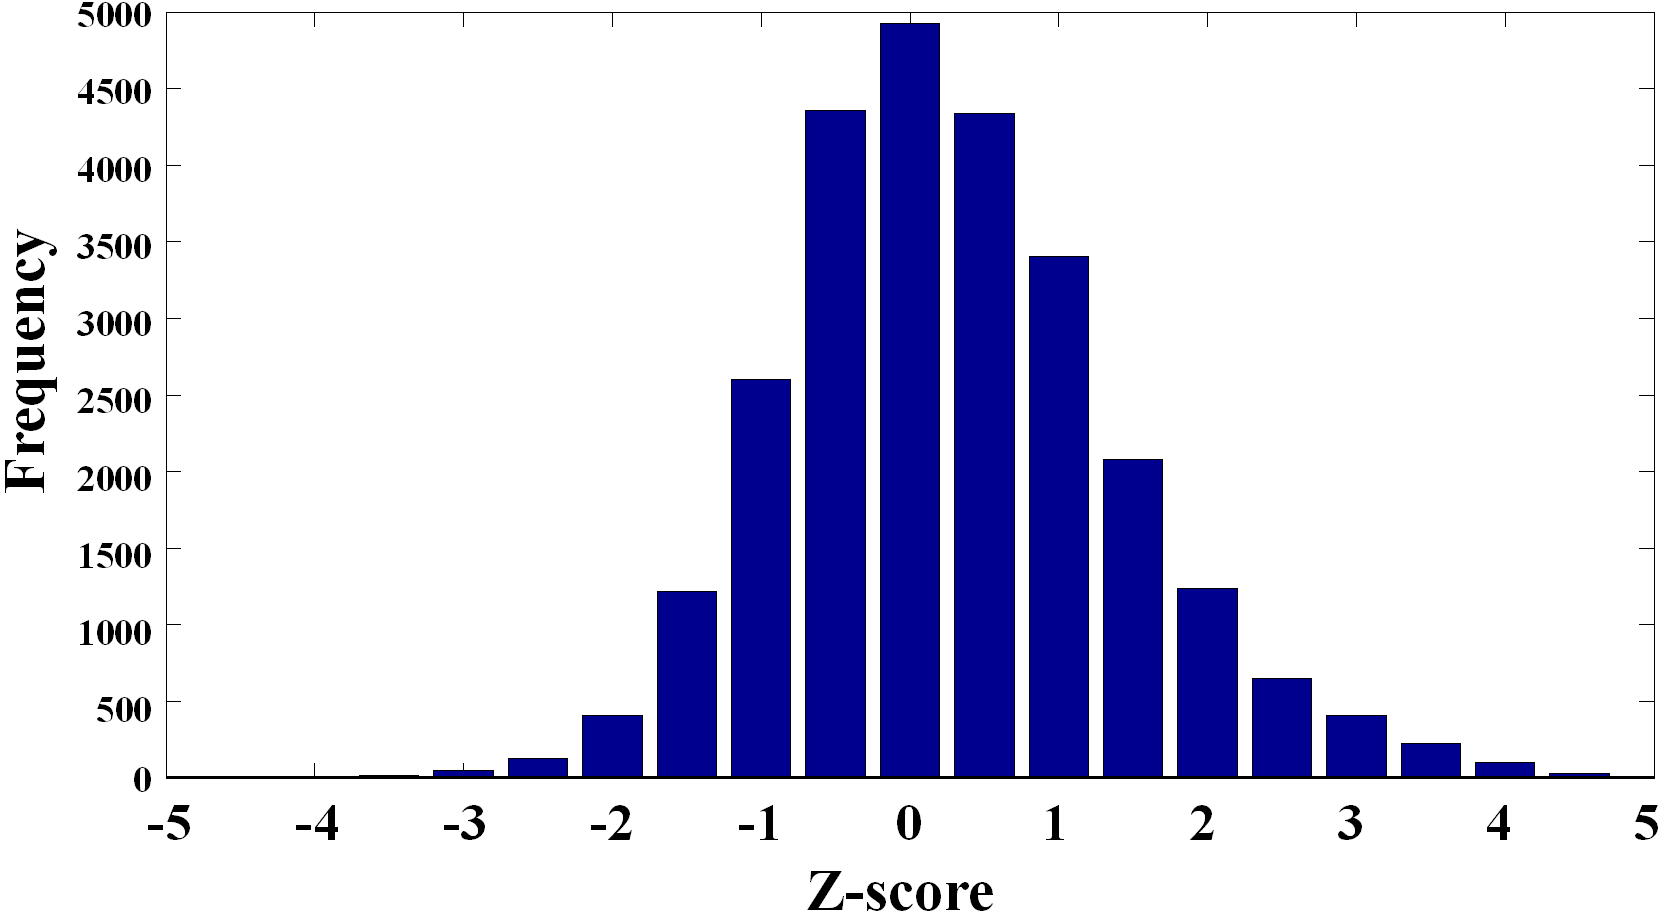
\includegraphics[width=2in] {figures/Z-Score-distribution.png}
%		\label{fig:distribution}
%	}
%	\caption{ Z-score distribution of city Sao Paulo, Brazil from Aug 1, 2012 to January 30, 2014 with time interval of five minutes. }
%	\label{fig:zscore-distribution}
%\end{figure}


\section{Algorithm}
\label{sec:algorithm}

\subsection{Graph Fourier Transform}
\label{sec:Graph_Fourier_Transform}
Given a signal $f$ defined on graph $\mathbf{G}$, its graph Fourier transform is considered as the projection of $f$ on the complete set of $\{\chi_l\}_{l=0}^{N-1}$, and is written as~\cite{hammond2011wavelets}:
\begin{equation}
\label{eq:Graph_Fourier_Transform1}
\hat{f}(l)=<\chi_{l},f>=\sum_{i=1}^{N}\chi^*_{l}(i)f(i)
\end{equation}
Since $\{\chi_l\}_{l=0}^{N-1}$ is complete, $f$ can be recovered by its graph Fourier transform coefficients $\hat{f}(l)$ as~\cite{hammond2011wavelets}:
\begin{equation}
\label{eq:Inverser_Graph_Fourier_Transform}
f(n)=\sum_{l=0}^{N-1}\hat{f}(l)\chi_{l}(n)
\end{equation}
Here, $\hat{f}(l)$ is the coefficient of component $\chi_l$.
\subsubsection{eigenvector $\chi_l$}
As an analog with classical signal processing, eigenvector $\chi_l$ is also referred to as
the  frequency of $\mathbf{G}$ by some researchers. In the latter part of this chapter, $\chi_l$ will be referred to as the eigenvector or frequency, alternatively. However, unlike the traditional frequency concept in classical signal processing fields, the frequency of $\mathbf{G}$ is a set of discreet vectors with length of $|V|$. Interestingly, like the classical signal Fourier transform, the
Parseval relation~\cite{shuman2015vertex} still holds, i.e.,
\begin{equation}
\label{eq:Parseval}
||\hat{f}||_2^2=||f||_2^2
\end{equation}
Equation~\ref{eq:Parseval} means that the
energy in the vertex domain and frequency domain is equal for any graph signal $f$. Without loss of generality, we assume $||f||_2 =1$.



\begin{figure}[h]
	\centering
    {
		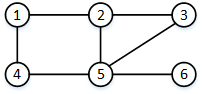
\includegraphics[height=1.4in] {figures/graph_G.png}
	}
	\caption{Graph $\mathbf{G_1}$, all edges's weight are $1$.}
	\label{fig:graph_G}
\end{figure}


\subsubsection{eigenvalue $\lambda_l$}
According to the definition of eigenvalue $\lambda_l$  in Equation~\ref{eq:eigenvalues}, the following equation holds:
\begin{equation}
\label{eq:lambda1}
\chi_{l}^T\lambda_{l}\chi_{l}=\chi_{l}^T\mathcal{L}\chi_{l}= \sum_{e_{mn}\in E} w_
{mn}[\chi_{l}(m)-\chi_{l}(n)]^2
\end{equation}Since $\chi_{l}$ is normalized, and $||\chi_{l}||_2 =1$, then,
\begin{equation}
\label{eq:lambda2}
\chi_{l}^T\lambda_{l}\chi_{l}=\lambda_l= \sum_{e_{mn}\in E} w_
{mn}[\chi_{l}(m)-\chi_{l}(n)]^2
\end{equation}
From equation~\ref{eq:lambda2}, we can see that $\lambda_l$ summarizes all the eigenvector deviations on any directly connected vertices $v_m$ and $v_n$ in $\mathbf{G}$. Since each term in the summation of the right-hand side is non-negative, the eigenvectors associated with smaller eigenvalues are smoother; i.e., the component differences between neighboring vertices are
small~\cite{shuman2015vertex}. As the eigenvalue increases, larger differences in neighboring
components of the graph Laplacian eigenvectors are present.
Hence, for larger $\lambda_l$, its corresponding eigenvector, $\chi_l(n)$, has larger deviation among connected vertices. According to the definition of Laplacian matrix $\mathcal{L}$, it is easy to verify that $\lambda_0=0$ since $\mathcal{L}\cdot\vec{\textbf{1}}= 0\cdot\vec{\textbf{1}}$, where $\vec{\textbf{1}}=\{1,1,1,...,1\}$, and $\chi_o(n)=\frac{\vec{\textbf{1}}}{\sqrt{N}}$. Thus, $\chi_o(n)=\frac{\vec{\textbf{1}}}{\sqrt{N}}$ means that $\chi_o(n)$ is constant on each vertex, and that
there is no deviation among any two vertices in $\chi_0(n)$. For this reason, $\chi_0(n)$ is considered as the least abnormal component of $\mathbf{G}$. Similarly, $\chi_{N-1}(n)$ is considered as the most abnormal component of $\mathbf{G}$.

Figure~\ref{fig:graph_G} shows an undirected graph $\mathbf{G_1}$ where each edge's weight is $1$. Figure~\ref{fig:frequency1} shows  $\mathbf{G_1}$'s six eigenvectors distributions along each vertex. We can see that
$\chi_0$ is constant on very vertex, and has the smallest deviations along each edge. $\chi_5$ has the largest deviations, and the difference of $\chi_5$ along each edge is larger than any other eigenvector on average.



\begin{figure}[t]
	\centering
	\subfigure[]{
		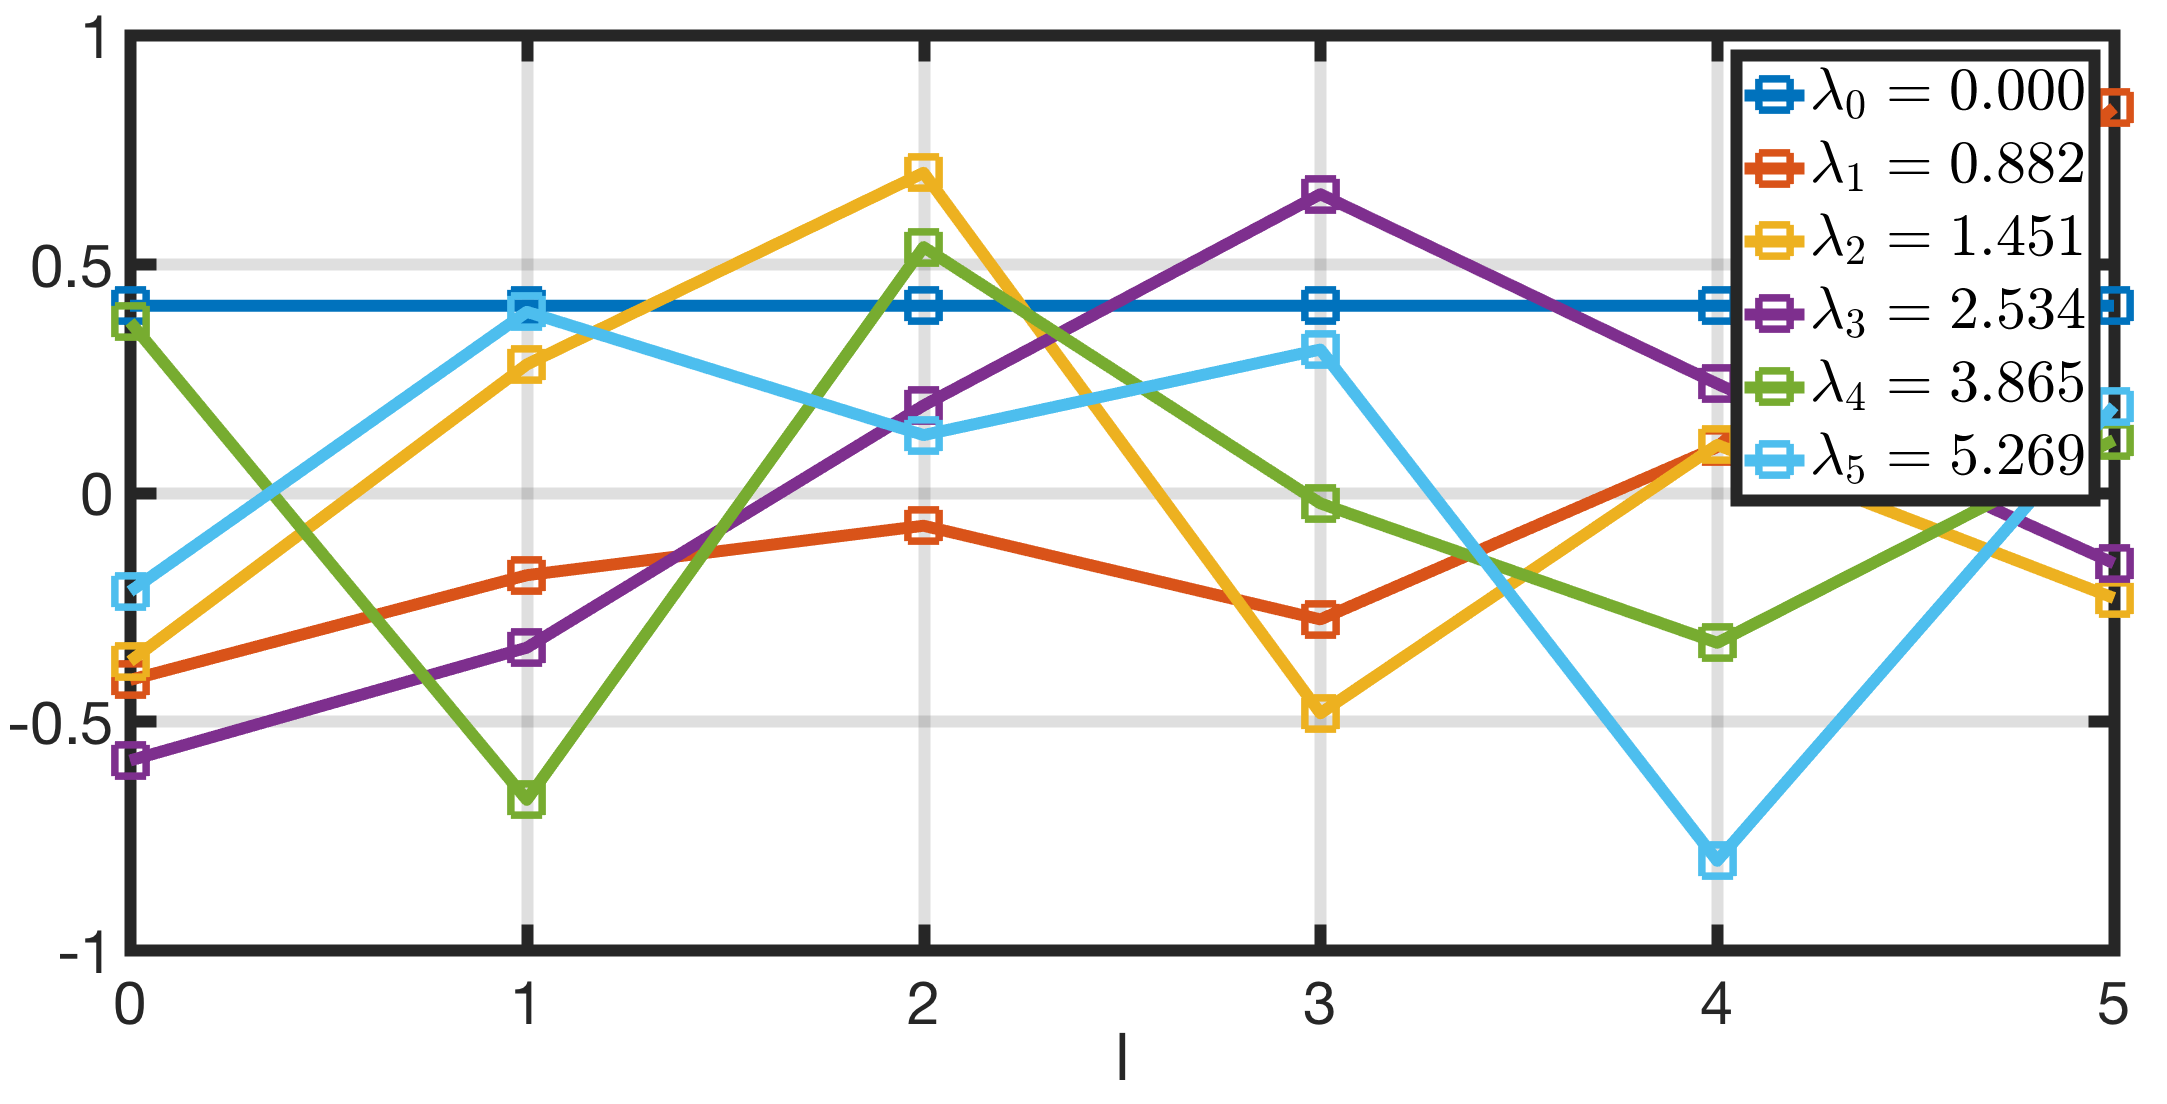
\includegraphics[width= 3in, height=1.5in] {figures/frequency.png}
		\label{fig:frequency1}
	}
	\subfigure[]{
		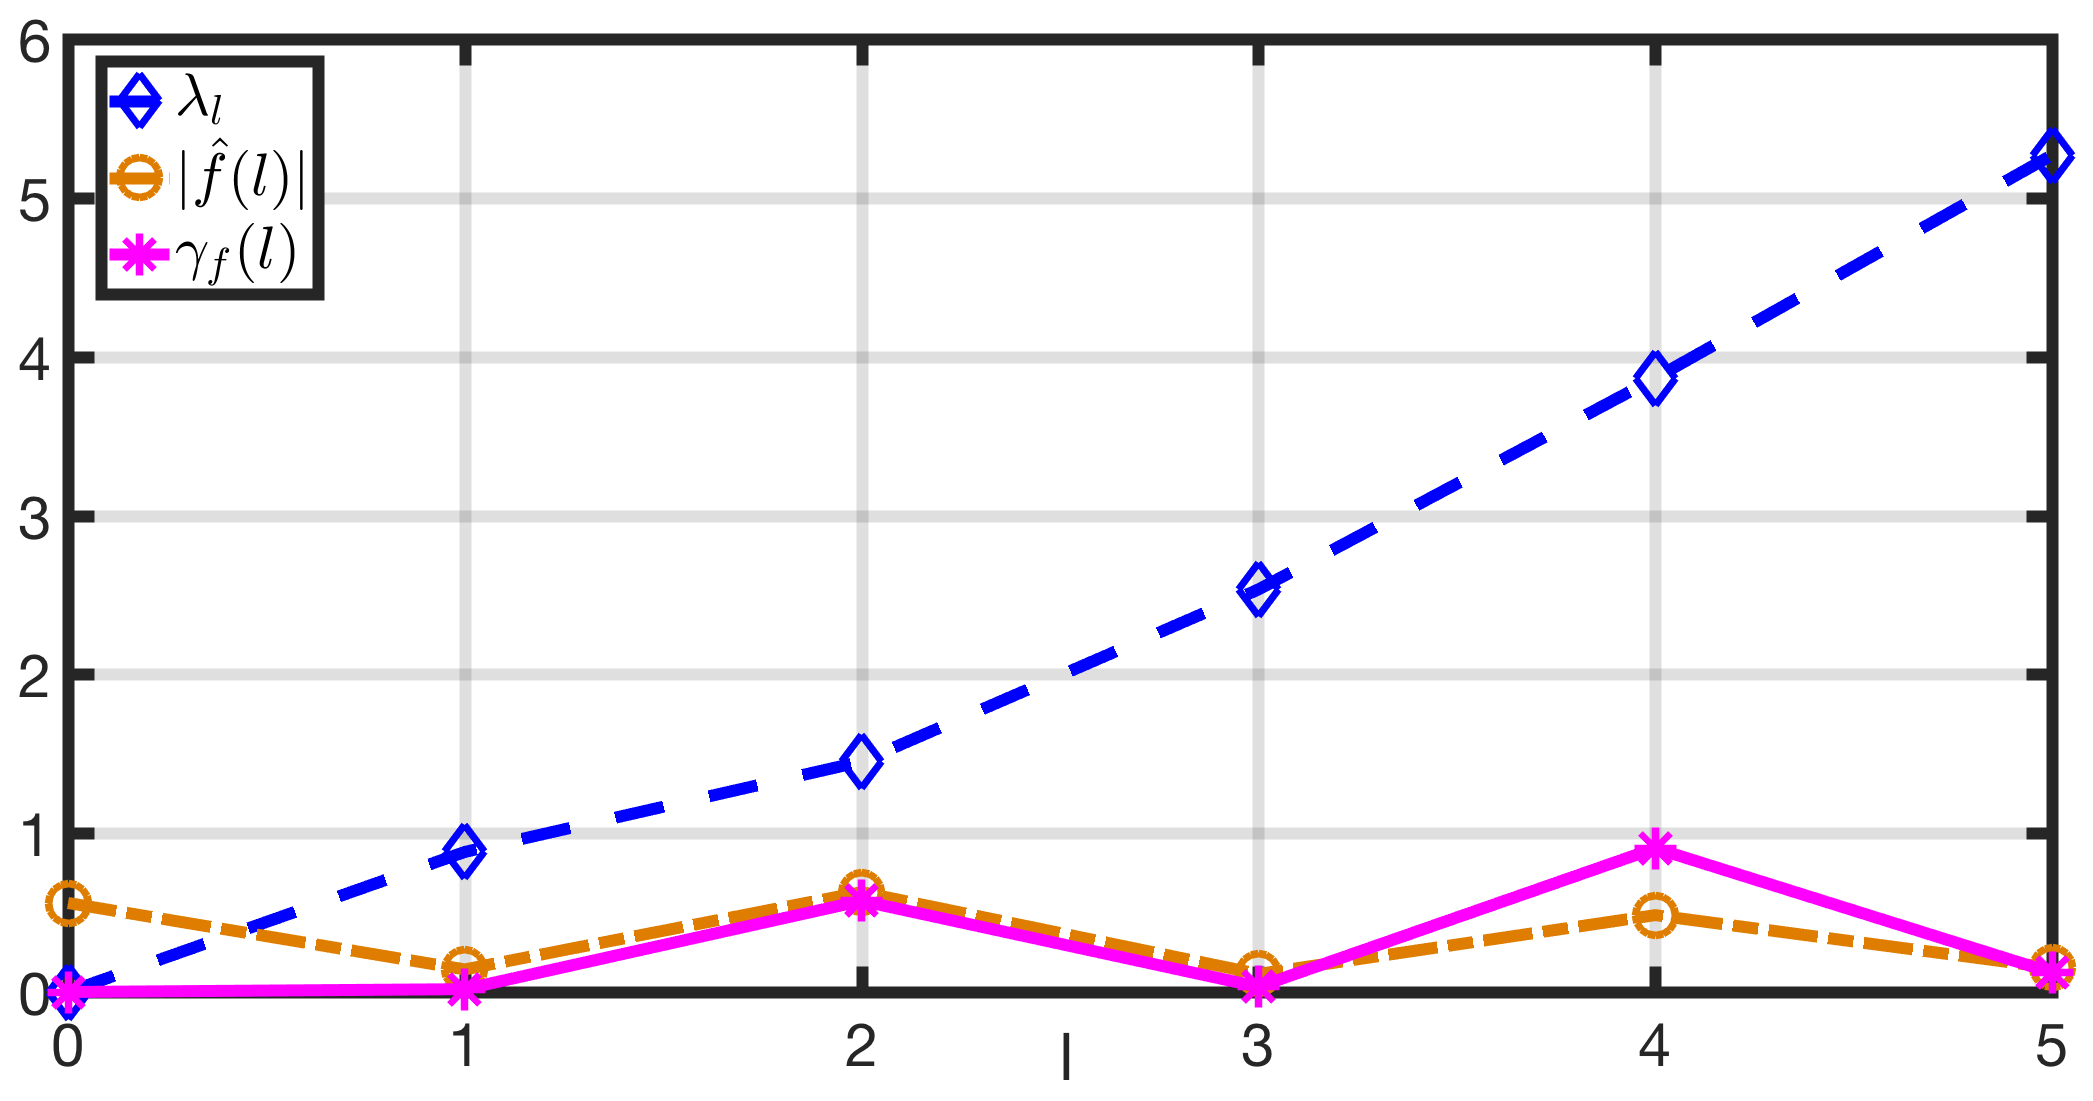
\includegraphics[width=3in, height=1.5in] {figures/g1_gamma.png}
		\label{fig:g1_gamma}
	}

	\subfigure[]{
		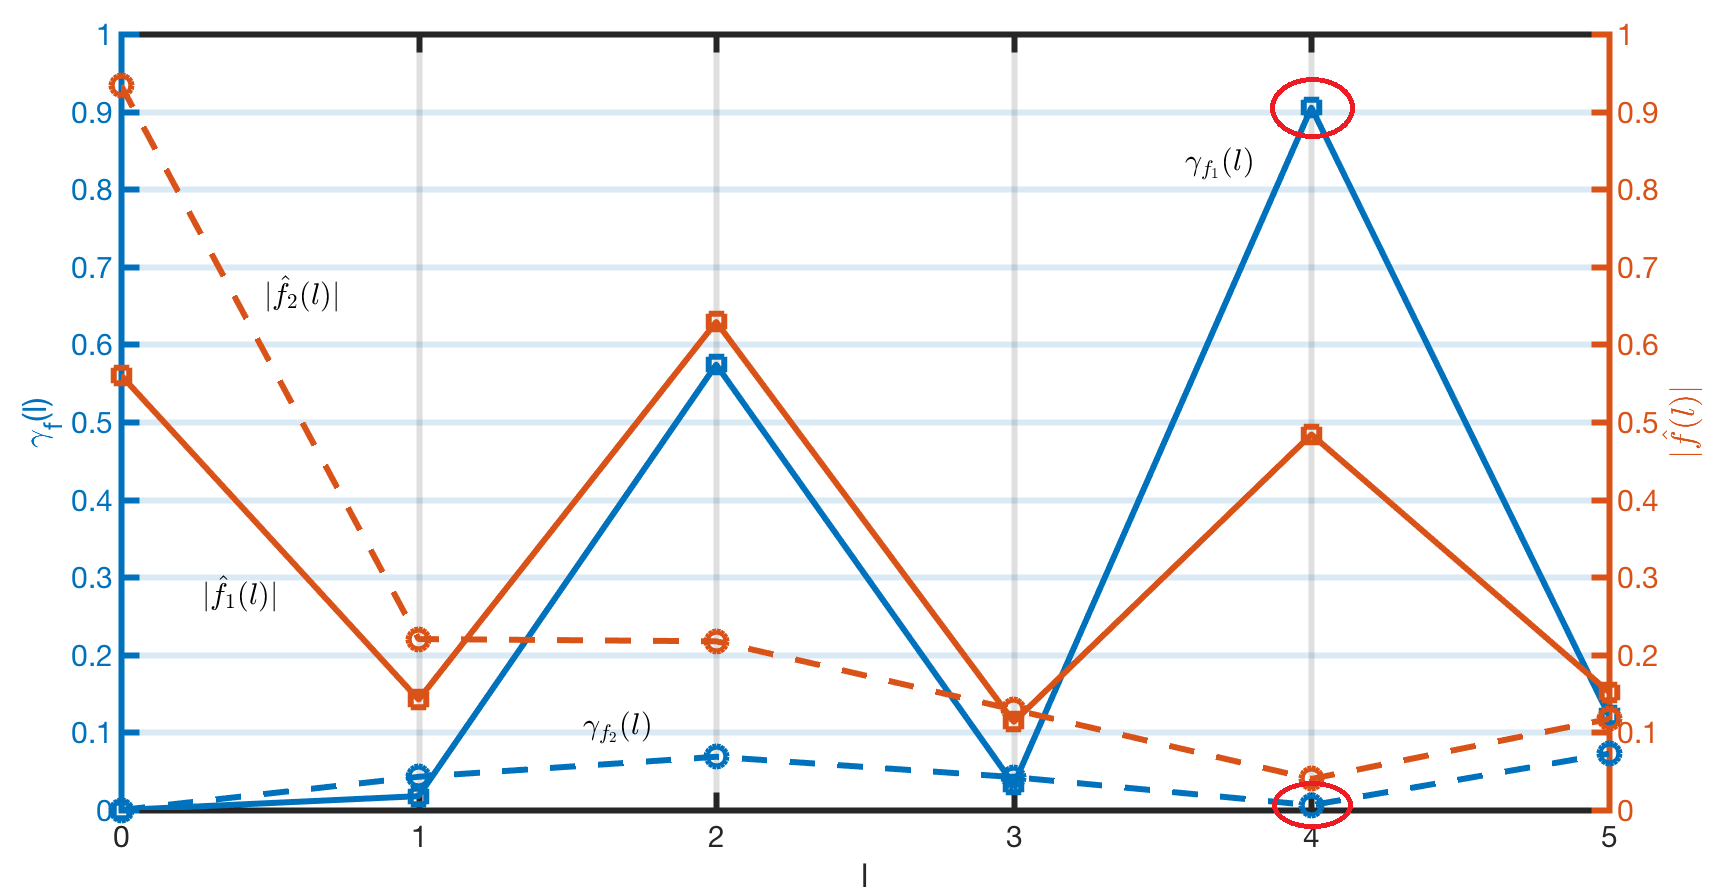
\includegraphics[width= 3.3in, height=1.5in] {figures/same_graph.png}
		\label{fig:same_graph}
	}

	\caption{(a): Eigenvector distribution along each vertex in graph $\mathbf{G_1}$.  (b): anomaly index $\gamma_f(l)$ of $f_1=[2,3,4,3,2,1]$ on graph $\mathbf{G_1}$. (c): anomaly index $\gamma_f(l)$ of $f_1=[2,3,4,3,2,1]$  and $f_2=[2,2,-3,4,3,1]$ on graph $\mathbf{G_1}$, where $\gamma_{f_1}=0.905$, and $\gamma_{f_1}=0.073$, labelled in red ovals.}
	\label{fig:f_on_g2}
\end{figure}






\begin{figure}[t]
	\centering
	\subfigure[$\mathbf{G_2}$]{
		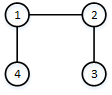
\includegraphics[height=1.1in] {figures/f_on_g1.png}
		\label{fig:scale1}
	}
	\subfigure[$\mathbf{G_3}$]{
		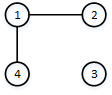
\includegraphics[height=1.1in] {figures/f_on_g2.png}
		\label{fig:scale2}
	}
	\caption{$f=[1,2,5,2]$ on two graphs $\mathbf{G_2}$ and $\mathbf{G_3}$.}
	\label{fig:f_on_g}
\end{figure}

\begin{figure}[t]
	\centering
    {
		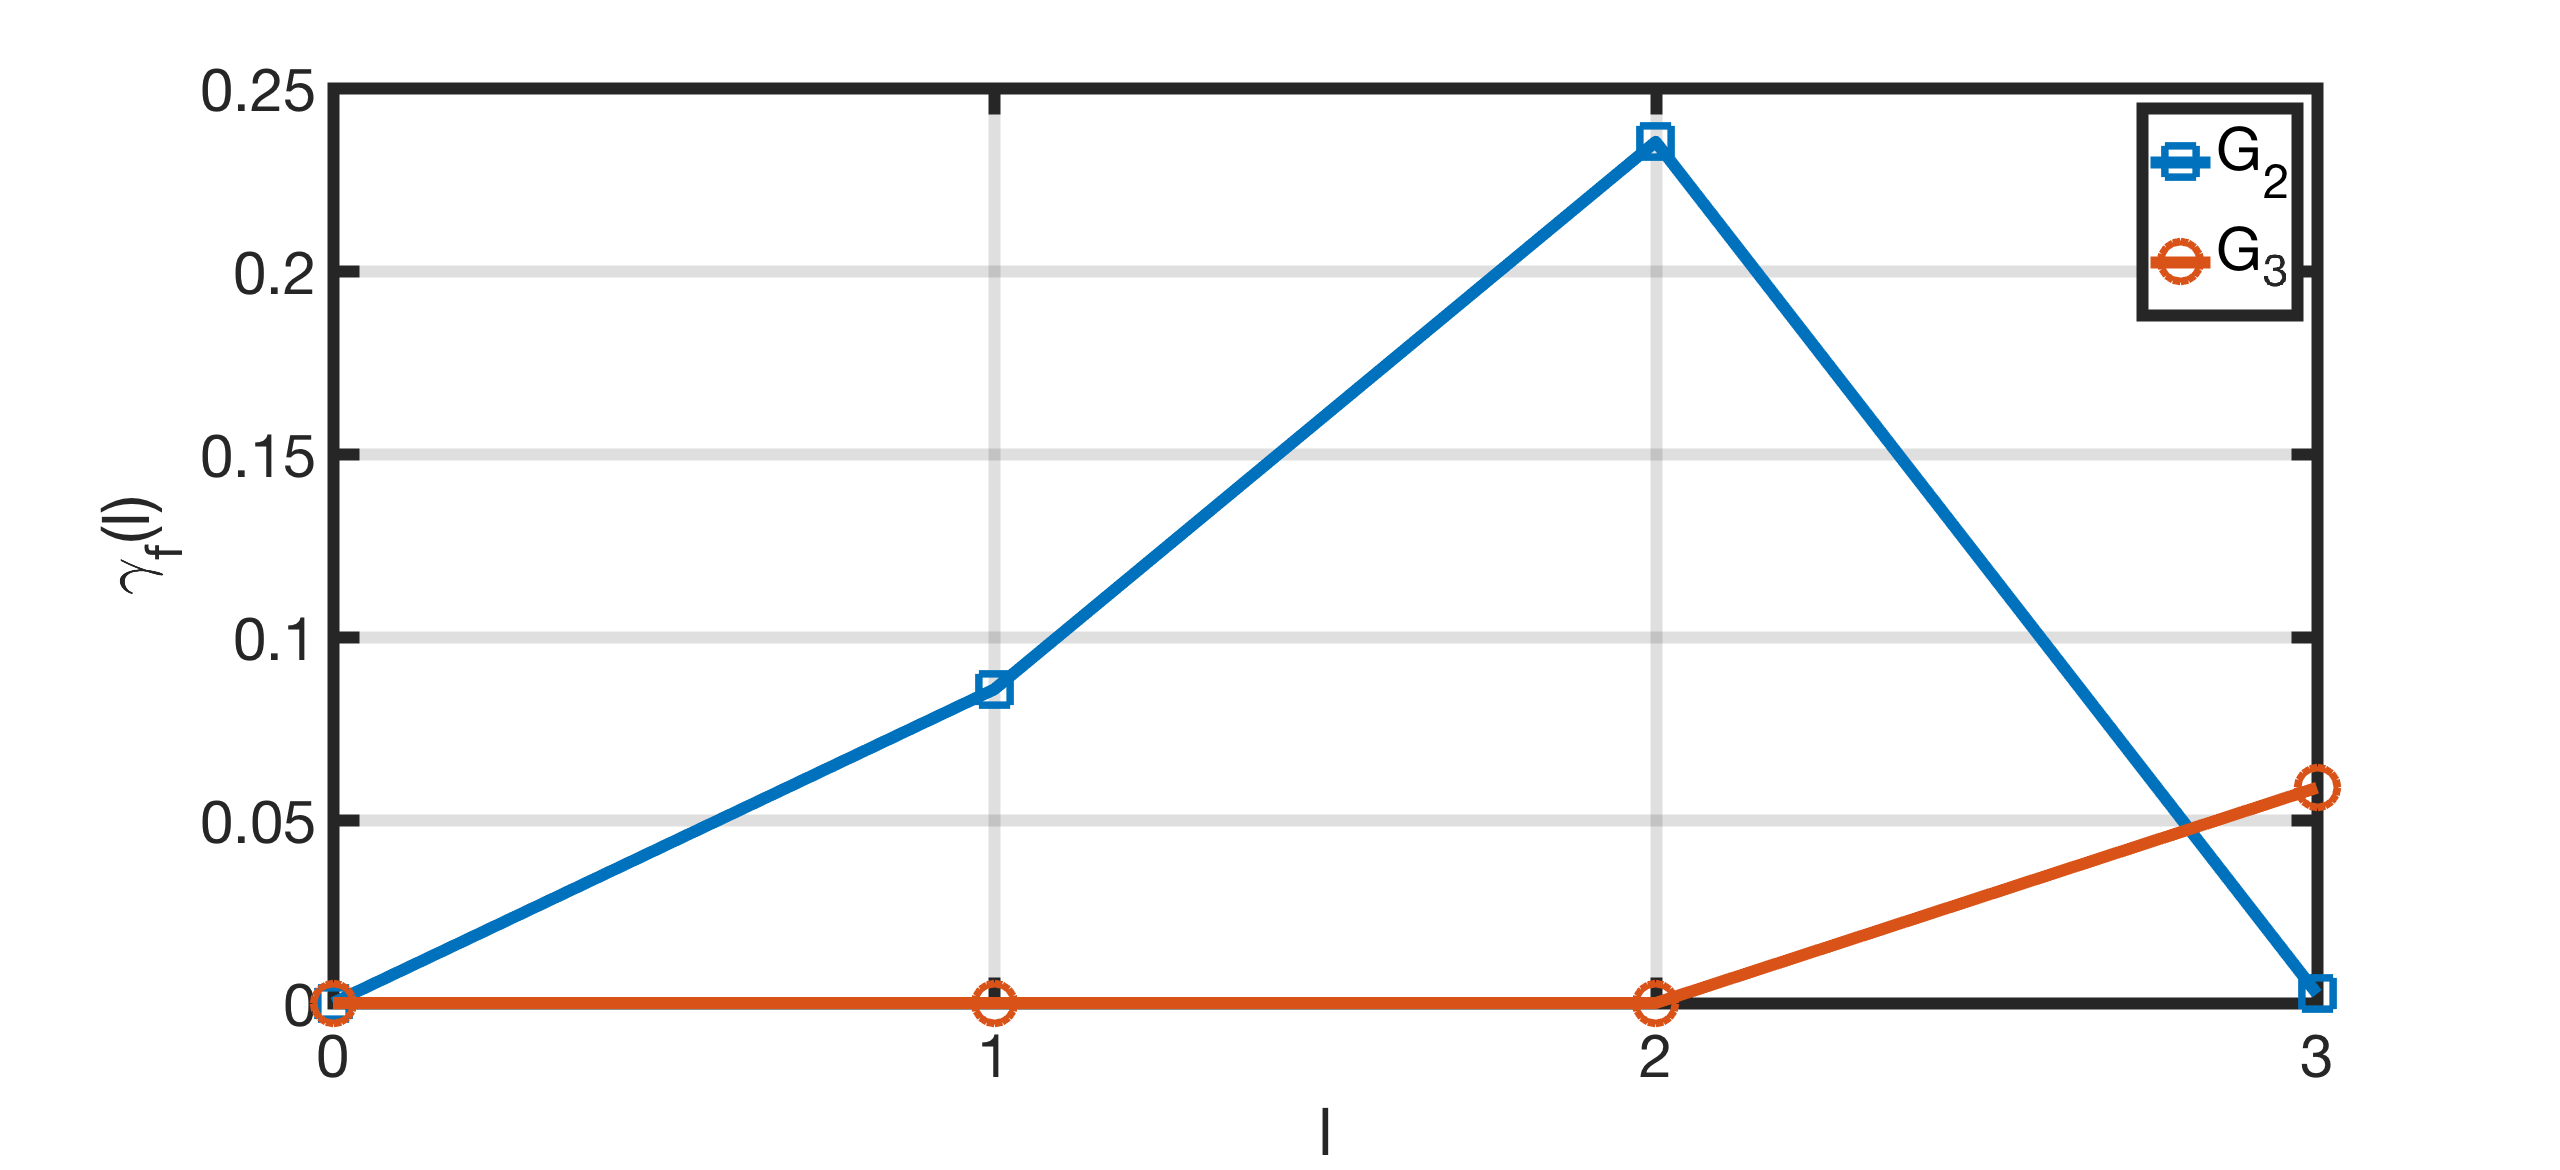
\includegraphics[width= 4in] {figures/new_graph.png}
		\label{fig:distribution2}
	}
	\caption{Anomaly indices of $\mathbf{G_2}$ and $\mathbf{G_3}$.}
	\label{fig:new_graph}
\end{figure}

\subsection{Global Anomaly Index}
\label{sec:signal_anomaly_on_Graph}

To quantify the anomaly of a vector $f$ defined on a graph $\mathbf{G}$, it's necessary to incorporate the intrinsic structures of $\mathbf{G}$ and $f$. As discussed above, $\hat{f}(l)$ represents the coefficient of frequency $\chi_l$, and $\hat{f}^2(l)$ is considered as the energy of frequency $\chi_l$. In addition, according to equation~\ref{eq:lambda2}, $\lambda_l$ represents the deviation of frequency $\chi_l$ along all the connected vertices. Therefore, in this chapter, we define the anomaly index of $\chi_l$ in $f$ as:
\begin{equation}
\label{eq:lambda3}
\gamma_f(l;\mathbf{G})=\lambda_l\hat{f}^2(l)= \lambda_l<f,\chi_l>^2
\end{equation}
$\gamma_f(l;\mathbf{G})$ depends on two parts, frequency $\chi_l$'s deviation sum $\lambda_l$, and its energy $\hat{f}^2(l)$. If the energy $\hat{f}^2(l)$ is small, even if $\lambda_l$ is large, the anomaly index of $\chi_l$ might be small. Obviously, $\gamma_f(0;\mathbf{G})$ is always $0$ since $\lambda_0=0$. Further, we use the maximal value of $\gamma_f(l;\mathbf{G})$ to represent the global anomaly of $f$ on $\mathbf{G}$:
\begin{equation}
\label{eq:lambda4}
\gamma_f(\mathbf{G})=\underset{0 \leq l \leq N-1}{\max}{\gamma_f(l;\mathbf{G})}.
\end{equation}
Here, $\gamma_f(l;\mathbf{G})$ refers to the anomaly extension of $\chi_l$ in $f$ defined on $\mathbf{G}$, instead of implying the anomaly extension of vertex $v_l$.
For brevity, $\gamma_f(l;\mathbf{G})$  and $\gamma_f(\mathbf{G})$ are shortened as $\gamma_f(l)$ and $\gamma_f$, respectively, when $\mathbf{G}$ is known.

Figure~\ref{fig:g1_gamma} plots the anomaly index $\gamma_f(l)$ of $f_1$ on graph $\mathbf{G_1}$, where $f_1=[2,3,4,3,2,1]$. The six markers on the dashed blue are the six eigenvalues of $\mathbf{G}$. The yellow line is $|\hat{f}(l)|$, and the pink line is the anomaly index, $\gamma_f(l)$ for frequency $\chi_l$. Because $\gamma_f(l)$ depends on both $\lambda_l$ and its power $\hat{f}^2(l)$, for the yellow line, even though $\chi_0$ has the strongest power, its deviation $\lambda_0 = 0$, thus $\gamma_f(0)=0$. On the other hand, $\chi_5$ has the largest deviation; but its power $|\hat{f}(5)|^2$ is small, which makes $\gamma_f(5)$ is also small. Considering the $\chi_4$ has a high deviation (eigenvalue) and a strong power of frequency, it has the largest anomaly index. To compare the influence of different $f$ on anomaly index, we show an example in Figure~\ref{fig:same_graph}. Setting $f_1=[2,3,4,3,2,1]$ and $f_2=[2,2,-3,4,3,1]$, we plot their anomaly index $\gamma_{f}$ and energy $|\hat{f}(l)|$ respectively.
The light blue curves stand for anomaly indices and the
yellow curves stand for $|\hat{f}(l)|$. The solid line stands for $f_1$, and the
dashed line stands for $f_2$. As we can see, for high frequency $\chi_l$, $f_1$ has a larger power than $f_2$, and hence a higher anomaly index than $f_2$, where $\gamma_{f_1}=0.905$ and $\gamma_{f_2}=0.073$. This is consistent with that $f_1$ has larger deviations than $f_2$.

As we discussed before, the anomaly index depends on graph structure and $f$. As shown in Figure~\ref{fig:same_graph}, different $f$ might have very different anomaly index because the power of $\chi_l$ distribution is different. Similarly, for the same signal $f$ on two different graphs, it might have very different anomaly indices. Figure~\ref{fig:f_on_g} shows two graphs with the same $f=[1,2,5,2]$. Figure~\ref{fig:new_graph} illustrates the anomaly index of $f$ on $\mathbf{G_2}$ and $\mathbf{G_3}$, where $\gamma_{f}(\mathbf{G_2})=0.073$ and $\gamma_{f}(\mathbf{G_3})=0.235$. (This is because in $\mathbf{G_3}$ because there is no edge connecting $v_2$ and $v_3$, the difference between $f(2)$ and $f(3)$ is not considered as an anomaly.)


{\textbf{Remarks:}}
In this subsection, we have introduced the anomaly index $\gamma_f(l;\mathbf{G})$ to measure the anomaly of $\chi_l$ in $f$ defined on $\mathbf{G}$ by combing the spectrum structure of $\mathbf{G}$ and $f$. $\gamma_f(l;\mathbf{G})$ depends on two parts: (1) the eigenvalue which reflects the deviations of $\chi_l$; (2) the $|\hat{f}(l)|^2$  which represents the power of $\chi_l$ in $f$. $\gamma_f(l;\mathbf{G})$ reflects the anomaly index of $\chi_l$. We use the maximal value of $\gamma_f(l;\mathbf{G})$ to define the anomaly index of $f$, which denotes the global anomaly index of $f$ on $\mathbf{G}$.



\begin{figure}[t]
	\centering
	\subfigure[]{
		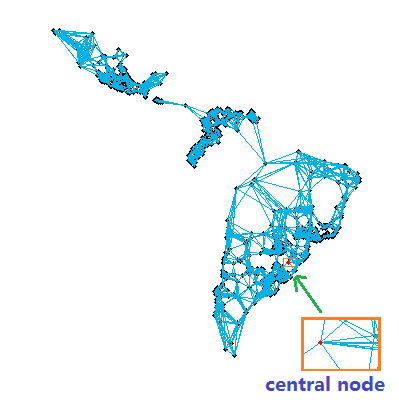
\includegraphics[height=1.8in] {figures/All-0.png}
		\label{fig:brazil1}
	}
	\subfigure[]{
		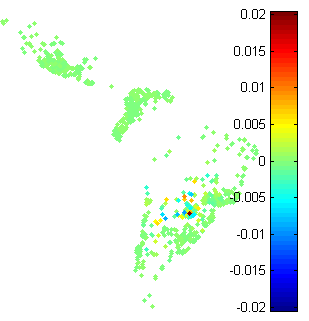
\includegraphics[height=1.8in] {figures/All-08.png}
		\label{fig:brazil2}
	}
		\subfigure[]{
		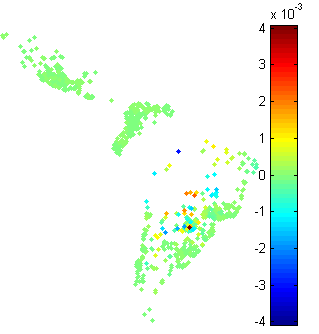
\includegraphics[height=1.8in] {figures/All-18.png}
		\label{fig:brazil3}
	}
	\subfigure[]{
		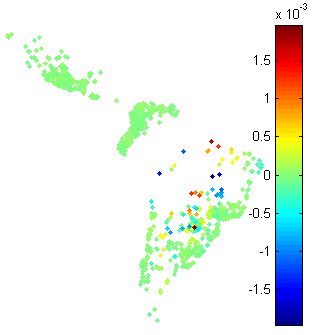
\includegraphics[height=1.8in] {figures/All-26.png}
		\label{fig:brazil4}
	}
    \subfigure[]{
		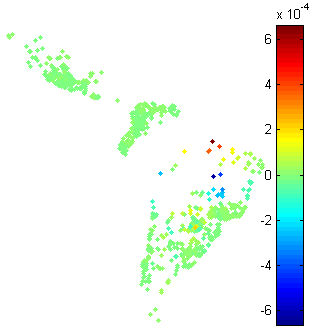
\includegraphics[height=1.8in] {figures/All-80.png}
		\label{fig:brazil5}
	}
	\subfigure[]{
		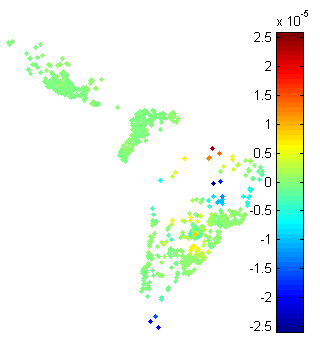
\includegraphics[height=1.8in] {figures/All-400.png}
		\label{fig:brazil6}
	}
	\caption{Spectral graph wavelet on South America. (a) vertex at which wavelets are centered in red dot. (b)-(f) wavelets, scales at 0.8, 1.8, 2.6, 8, and 40 respectively.}
	\label{fig:southamericanscale}
\end{figure}



\subsection{Graph Wavelets}
\label{sec:graph_wavelet}
Classic wavelet formalisms have been referred to as mathematical microscopes because of their capability to depict
signal anomalies at different scales. In the case of complex networks, graph wavelets render the graph with good localization properties both in frequency and vertex (i.e. spatial) domains. Their scaling property allows us to zoom in/out of the underlying structure of the graph.

%It is useful to analyze $f$ by taking into account the intrinsic geometric structure of the graph $\mathbf{G}$. In order to identify and exploit structure of  $f\in \mathbb{R}^N$, the spectral graph $\sigma({\mathcal{L}}):=\{\chi_l\}_{l=0}^{N-1}$ can be used as a dictionary of atoms~\cite{shuman_ACHA_2013}. Thus, $f$ can be decomposed as a linear combination of $\{\chi_l\}_{l=0}^{N-1}$ as
%\begin{equation}
%\label{eq:graph_fourier}
%f(n)= \sum\limits_{l=0}^{N-1}\hat{f}(l)\chi_l(n)
%\end{equation}
%, where
%\begin{equation}
%\label{eq:graph_fourier1}
%\hat{f}(l):= \sum\limits_{n=0}^{N-1}\chi^*_l(n)f(n)
%\end{equation}
%$\chi_l$ is called the Fourier frequency of $f(n)$ based on the graph $\mathbf{G}$, and $\hat{f}(l)$ is the corresponding Fourier coefficient.
%Equation~\ref{eq:graph_fourier1} and Equation~\ref{eq:graph_fourier} are called Fourier transform and inverse Fourier transform, respectively.
%Equation~\ref{eq:graph_fourier1} gives a clear representation of the Fourier components in $f(n)$.
Recall that, from Equation~\ref{eq:Graph_Fourier_Transform1}, the anomaly pattern $\hat{f}(l)$ represents the anomaly components of $f$ from the whole graph perspective. However, information concerning the vertex-location cannot be identified from the Fourier transform. To address this issue, Hammond et al.~\cite{hammond2011wavelets} proposed constructing wavelet transforms functions over the vertices using weighted graphs, described in the following steps:

\begin{enumerate}
\item Define a continuous generating kernel functions $g(x)$ on $\mathbb{R}^+$;
\item Then, select a central vertex $a \in {V}$ and scale $s$, set the frequency coefficients as $g(s\lambda_l)\chi^*_l(a)$ for each frequency component $\chi_l$;
\item Finally, sum up all those frequency components $\chi_l$.
\end{enumerate}
In this way, the graph wavelet at central vertex $a$ is constructed as:
\begin{equation}
\label{eq:graphwaveletdefinition}
\psi_{s,a}(n) = \sum\limits_{l=0}^{N-1}g(s\lambda_l)\chi_l^*(a)\chi_l(n)
\end{equation}




After setting up the graph wavelet, the wavelet coefficients for $f$ can be defined as
\begin{equation}
\label{eq:graph_graphwavelet}
W_f(s,a)=<\psi_{s,a}, f>=\sum\limits_{l=0}^{N-1}g(s\lambda_l)\hat{f}(a)\chi_l(n)
\end{equation}
Similar to classical wavelets, graph wavelets obey following three properties, which are presented in detail in~\cite{hammond2011wavelets}.
 \begin{enumerate}
 \item \textbf{Reconstruction.}
 When the kernel function $g(x)$ satisfies the admissibility condition and $g(0)=0$,  $f(n)$ can be reconstructed by the wavelet coefficients.
\item \textbf{Discretization and Wavelet Frames.} For practical applications, the
scale $s$ of graph wavelet $\psi_{s,a}$ should be sampled with a finite number of scales. Given a real valued function $h(x)$ satisfying
\begin{equation}
\hat{h}(\omega) = \sqrt{\int_\omega^\infty\frac{|\hat{g}(\omega')|^2}{\omega'}d{\omega'} },
\end{equation}
where $\hat{g}$ and $\hat{h}$ are the classical Fourier transform of $g(x)$ and $h(x)$, the scaling function $\phi_{a}(n)$ can be generated as:
\begin{equation}
\label{eq:graphscaledefinition}
\phi_{a}(n) = \sum\limits_{l=0}^{N-1}h(\lambda_l)\chi_l^*(a)\chi_l(n)
\end{equation}
Accordingly, the scaling coefficients are defined as
\begin{equation}
S_f(a)=<\phi_a,f>
\end{equation}
Using scale set $\Theta:=\{s_j\}_{j=1}^J$, the discretized graph wavelet set $\{\psi_{s_j,a}\}_{j=1}^{J}$ $_{a=0}^{N-1}$, and scaling function set $\{\phi_a\}_{a=0}^{N-1}$ constitute a frame~\cite{hammond2011wavelets}.
According to frame theory~\cite{daubechies1992ten}, $f\in \mathbb{R}^N$ can be reconstructed from those $NJ+J$ wavelet and scaling coefficients as
\begin{equation}
\label{eq:frame}
f(n)=\sum_{a=v_0}^{v_{N-1}}[\sum_{j=1}^{J}W_{f}(s_j,a)\psi_{s,a}(n)+S_f(a)\phi_{a}(n)].
\end{equation}For brevity, we assume that
\begin{equation}
\phi_a(n)=\psi_{s_0,a}(n),
\end{equation} and
\begin{equation}
S_f(a)=W_f(s_0,a).
\end{equation}Therefore, equation~\ref{eq:frame} can be written as
\begin{equation}
\label{eq:frame2}
f(n)=\sum_{a=v_0}^{v_{N-1}}\sum_{j=0}^{J}W_{f}(s_j,a)\psi_{s,a}(n).
\end{equation}In the later part of this chapter, we do not differentiate between
scaling coefficient and wavelet coefficient.
A detailed algorithm and treatment concerning the choice of $\Theta$ can be found in~\cite{hammond2011wavelets}.




\begin{figure*}[t]
	\centering
	\subfigure[wavelet $\psi_{s_1,a}$]{
		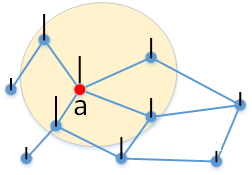
\includegraphics[width=1.4in, height=1.1in] {figures/wavelet1.png}
		\label{fig:scale1}
	}
	\subfigure[wavelet $\psi_{s_2,a}$]{
		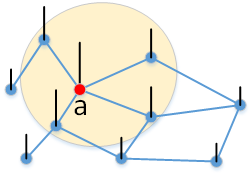
\includegraphics[width=1.4in, height=1.1in] {figures/wavelet2.png}
		\label{fig:scale2}
	}
\subfigure[$f(n)$ vs vertices]{
		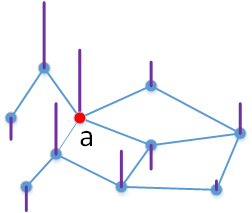
\includegraphics[width=1.4in, height=1.1in] {figures/wavelet3.png}
		\label{fig:scale3}
	}
\subfigure[$W'_f(s,a)$ vs scale $s$]{
		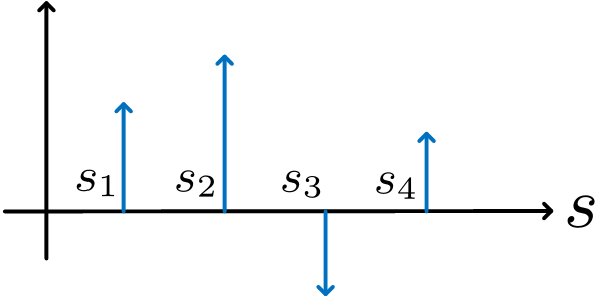
\includegraphics[width=1.5in, height=1.1in] {figures/wavelet4.png}
		\label{fig:scale4}
	}
	\caption{Graph wavelet scale and graph wavelet coefficient.}
	\label{fig:graphwaveletscale}
\end{figure*}



\item \textbf{Localization in vertex domains.} Given a central vertex $v_a$ and its graph wavelet $\psi_{s,a}(n)$, suppose the kernel function $g$ is $K+1$ times continuously differentiable, let $v_n$ be an vertex of $\mathbf{G}$ with $d_G(n,a)>K$, then there exists constants $D$ and $\beta$, such that
\begin{equation}
\label{equ:waveletbound}
\frac{|\psi_{s,a}(n)|}{||\psi_{s,a}||}\leq D \beta
\end{equation} for all $s<\beta$.
$d_G(n,a)$ is the shortest path distance, which is the minimum number of edges in any path that connect vertices $v_n$ and $v_a$~\cite{hammond2011wavelets}. Equation~\ref{equ:waveletbound} shows for any vertex $v_n$ that is far away from center vertex $v_a$ ($d_G(n,a)>K$), $\frac{|\psi_{s,a}(n)|}{||\psi_{s,a}||}$ is upper bounded by $D\beta$. In other words, for vertex $v_n$ which is far away form vertex $v_a$, its wavelet value is linearly attenuated by scale $s$.  When the scale $s$ is small, their wavelet value of marginal vertices will be vanished quickly. The marginal vertices are those which satisfy equation~\ref{equ:waveletbound}. All the other vertices are called kernel vertices, denoted by $\mathcal{K}(s,a)$. Obviously, $\forall v_n \in \mathcal{K}(s,a)$,  $d_G(n,a)\le K$. Thus $\mathcal{K}(s,a)$ is automatically compact.
Figure~\ref{fig:graphwaveletscale} shows two graph wavelets centered on the same vertex $a$, but with two different scales, $\psi_{s_1,a}$ and $\psi_{s_2, a}$, where $s_1<s_2$. The length of the vertical bar on each vertex denotes its graph wavelet value. The highlighted areas denote the kernel vertices ($d_G(n,a)\le 1$), and the others are marginal vertices. We can see that the wavelet values on marginal vertices in Figure~\ref{fig:scale1} are smaller than those in Figure~\ref{fig:scale2}. Figure~\ref{fig:scale3} is $f$'s distribution along each vertex, and Figure~\ref{fig:scale4} shows the wavelet coefficients with center node $a$ for different scales, which indicates that
$W_f(s_2,a)$ has the largest value, and $W_f(s_3,a)$ with the smallest.
 \end{enumerate}





% {\textbf{Remarks:}} Essentially, the wavelet frame is generated by kernel function $g(x)$ and scaling function $h(x)$ with $J$ different scales. Those functions are also called filter banks. Figure~\ref{fig:brazil_filter} shows the wavelet filter banks for Brazil graph which we will mention in the experiment part.

% \begin{figure}[h]
% 	\centering
%     {
% 		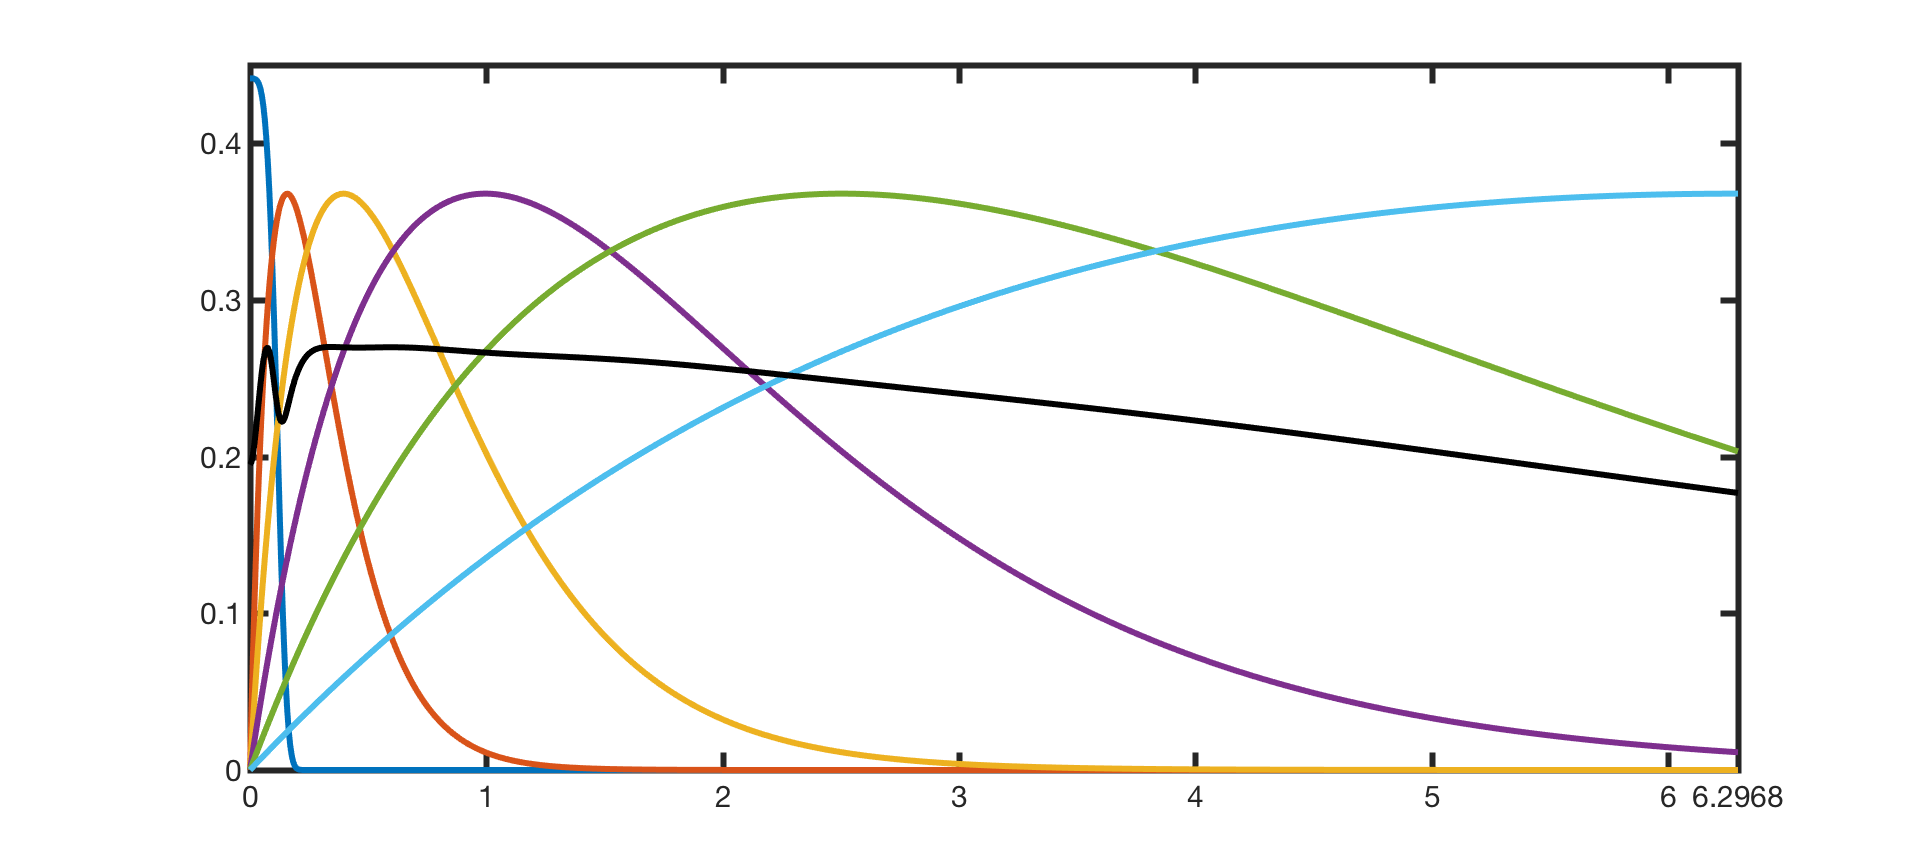
\includegraphics[width= 3.2in] {figures/brazil_filter.png}
% 		\label{fig:distribution2}
% 	}
% 	\caption{Wavelet filter banks for Brazil graph.}
% 	\label{fig:brazil_filter}
% \end{figure}



\subsection{Group Anomaly Detection via Graph Wavelets}
\label{sec:Group_Anomaly_Detection_via_graph_wavelet}
According to Equation~\ref{equ:waveletbound}, when $s$ is small, the weights of the marginal vertices are severely attenuated.
Essentially, $W_f(s,a)$ is equivalent to the sum of $f$ with large weights on kernel vertices, and small weights on marginal vertices.
%, and can also be treated as a similarity between $f$ and $\psi'_{s,a}$.
When $f$ is of uniformly large negative/positive values on kernel vertices, then $W_f(s,a)$ will be a large negative/positive value with scale $s$.

The localization property of graph wavelets makes them appropriate for group anomaly detection since they automatically identify the kernel vertices from marginal vertices. These kernel vertices form a compact subset since each one of them is close to the same center vertex $a$, which avoids the compactness constraint condition in Equation~\ref{eq: problem_conventional}, thus reducing
its computational complexity greatly. We propose our group anomaly detection algorithm based on graph wavelets in Algorithm~\ref{algo:event_detection1}. It iterates $NJ+J$ times, and each iteration selects a vertex as the center node, and computes the wavelet coefficient $W_f(s_j, a)$ with $J+1$ scales. When $W_f(s_j, a)$ is larger than some pre-set threshold $\omega_{th}$, it considers the corresponding kernel vertices, $\mathcal{K}(a)$, as an abnormal burst group. Similarly, when $W_f(s_j, a)$ is smaller than $-\omega_{th}$, it considers $\mathcal{K}(a)$ as an abnormal absenteeism group. The computational complexity is $O(J|V|^2)$.

\begin{algorithm}[t]
\centering
\captionsetup{font=scriptsize}
\caption{Group Anomaly Detection using Graph Wavelets}
{\footnotesize \begin{algorithmic}[1]
\STATE {\bf Input:} graph and absenteeism score vector $\mathbf{G}(V,E;f^l)$ at time interval $l$, wavelet threshold $\omega_{th}$.
\STATE {\bf Output:} abnormal burst group set $\mathcal{I}^{bur}$ and absenteeism group set $\mathcal{I}^{abs}$.	\STATE{compute graph spectrum $\sigma{(\mathbf{G})}$};
\STATE{set graph wavelets $\psi_{s,a}(n)$ and scales set $\{s_j\}_{j=0}^J$ for all $a\in V$};
\FORALL {center node $a\in V$ and $s_j \in \{s_j\}_{j=0}^J$}
	    \STATE{compute $W_f(s_j, a)$};
		\IF {$W_f(s_j, a) \ge \omega_{th}$}
		    \STATE{add group $\mathcal{K}(s_j,a)$ to $\mathcal{I}^{bur}$}
	    \ENDIF
	
		\IF {$W_f(s_j, a)\le -1*\omega_{th}$}
		    \STATE{add group $\mathcal{K}(s_j,a)$ to $\mathcal{I}^{abs}$}
	    \ENDIF	
	
\ENDFOR	
\RETURN {abnormal burst group $\mathcal{I}^{bur}$ and absenteeism group set $\mathcal{I}^{abs}$.}
\end{algorithmic}}
\label{algo:event_detection1}
\end{algorithm}


{\textbf{Remarks:}}
\begin{enumerate}
\item Graph wavelets form a frame where the function $f$ can be reconstructed by their coefficients.
As long as the scale level $J$ is high enough, $f$ can be well decomposed into the frame basis. Thus, using graph wavelets to exploit the structure of functions defined on graphs is much more reasonable.
\item Graph wavelets transform selected kernel vertices, $\mathcal{K}(s,a)$, that are close to the central vertex $a$, and attenuate the impact of other marginal vertices that are far away from $a$. The abnormal group selected by graph wavelet approach is automatically compact, and circumvent high computational complexity, which makes is easily adaptable to a wide variety of application scenarios.
\item Graph wavelets are able to identify abnormal burst groups and absenteeism groups simultaneously without extra computation cost.
\end{enumerate}




%\subsection{Group Absenteeism Event Detection}
%\label{sec:Group Absenteeism Event Detection}
%In our real world, there are various scenarios that causes people's silent on the social media for a certain amount of time. Take Earthquake emergence for example, when earthquake is happening, people hardly get a chance to use social media ( communication infrastructure might be paralyzed), thus it causes twitter volume in the affected area anomaly low. Some other examples, like flooding, blackout, and so on, often bring about similar phenomena. We call this kinds of events as absenteeism event. When absenteeism event is over, and people's circumstance is recovered to normal, it follows some kind of burst in social media since it's natural for people to talk about their experience concerning the absenteeism event. Usually, the severer of the absenteeism event is, the stronger absenteeism of the social media may present during the even, and the stronger burst will follow after.
%
%We propose a novel two-pass absenteeism based event detection algorithm. The underlying rationale of this algorithm is based on the following concepts.
%\begin{enumerate}
%\item At time interval $l$, using algorithm~\ref{algo:event_detection1} to identify absenteeism groups. For each absenteeism group $\mathcal{K}(s_j,a)$, it search burst groups $\mathcal{K}(s_k,b)$ which happens within a time window $L$. We claim that the time delay between $\mathcal{K}(s_j,a)$ and $\mathcal{K}(s_k,b)$ should be smaller than $L$, if the former is caused by the latter. When the time delay is larger that some pre-set $L$,  we claim that the burst group and the absenteeism group are uncorrelated.
%\item $\mathcal{K}(s_j,a)$ and $\mathcal{K}(s_k,a)$ should also be geographically correlated. This is because people are more likely to pay attention to events around where they live. To mathematically measure the geographically closeness of two city sets $\mathcal{K}(s_j,a)$ and $\mathcal{K'}(s_k,b)$, we define closeness $\rho(\mathcal{K}(a),\mathcal{K'}(b))$ as
%\begin{equation}
%\label{eq:eventsimilarity}
%\rho(\mathcal{K}(s_j,a),\mathcal{K'}(s_k,b)) = \frac{|\mathcal{K}(s_j,a)\cap\mathcal{K'}(s_k,b)|}{|\mathcal{K}(s_j,a)|\cdot|\mathcal{K'}(s_k,b)|}
%\end{equation}, where $|\mathcal{K}(\cdot)|$ is the city number. When $\rho$ is above some threshold $\rho_{th}$, we infer that an absenteeism event occurred and that it evolved on social networks into distinct phases: first group absenteeism, followed by a spike or burst in user activity. We denote this absenteeism event as e$\{\mathcal{K}(s_j,a),\mathcal{K}(s_k,b),\tau\}$, $\tau$ is the time delay.
%\item The computational complexity is $O(|\mathcal{I}^{bur}|\cdot |\mathcal{I}^{abs}|\cdot L\cdot |V|)$, and is $O(L|V|^3)$ in worst cases.
%%For instance, taking the power-cut-off for instance, usually only people who live in the affected area will ``yield at " this event a lot because it brings inconvenience to their life. However, people who live outside of the affected areas would hardly mention this event. Thus, to measure the correlation between absenteeism pattern and burst pattern is proposed as:
%\end{enumerate}
%
%\noindent\textbf{Remarks:}
%
%\noindent{In our real world, there are some absenteeism events, for example natural disasters (earthquake, flooding, electricity outage), generates absenteeism group and then burst group in social network. We propose the two-pass algorithm to detect those absenteeism events based on the assumption that those absenteeism and burst groups have strong correlation, spatially and temporally}.
%
%
%\begin{algorithm}[t]
%\centering
%\captionsetup{font=scriptsize}
%\caption{Two-Pass Absenteeism Event Detection}
%{\footnotesize \begin{algorithmic}[1]
%\STATE {\bf Input:} graph and absenteeism score vector $\mathbf{G}(V,E;f^l)$ at time interval $l$, and time window size $L$.
%\STATE {\bf Output:} absenteeism event set $\mathcal{E}$.	
%\STATE{compute burst group set $\mathcal{I}^{bur}$ by algorithm~\ref{algo:event_detection1}};
%		    	\FORALL {$\tau$ from $l+1$ to $l+L$}
%		    	    \STATE{compute absenteeism group set $\mathcal{I}^{abs}$ by algorithm~\ref{algo:event_detection1}};
%		    	    \FORALL {$\mathcal{K}(s_j,a)\in \mathcal{I}^{bur}$ and $\mathcal{K'}(s_k,b)\in \mathcal{I}^{abs}$}
%				    	    		
%		    	    		    \IF {$\rho(\mathcal{K}(s_j,a),\mathcal{K'}(s_k,b))\ge \rho_{th}$}
%		    	    		    \STATE{add absenteeism event $e\{\mathcal{K}(s_j,a),\mathcal{K}(s_k,b),\tau\}$ to $\mathcal{E}$}
%		    	    	    	\ENDIF
%
%                   \ENDFOR
%
%	            \ENDFOR	
%		
%
%
%\RETURN {absenteeism event set $\mathcal{E}$}.
%\end{algorithmic}}
%\label{algo:event_detection}
%\end{algorithm}







\section{Experimental Results}
\label{sec:experiment}
This section discusses the applications of our approach for detecting group anomaly.
We begin by briefly describing the dataset we use for our experiments in Section~\ref{sec:data_collection}.
Then we discuss in Section~\ref{sec:experimental_setup} the implementation details of how we assemble the graph $\mathbf{G}$ and construct the graph wavelets $\psi_{s,a}$.
After that, we present group anomaly detection performance in protest events detection. In Section~\ref{sec:highlighted_results}, we describe three case studies that illustrate how the graph wavelet is able to capture to absenteeism events like disaster scenarios.


\subsection{Data Collection and Preprocessing}
\label{sec:data_collection}
The study described in this chapter uses tweets from 22 countries in Latin America that were collected over 2 years (Jan 2012 to June 2014).
We query Datasift's streaming API to collect these tweets that also have meta-information including geotag bounding boxes (structured geographical coordinates), Twitter Places (structured data), user profile location (unstructured, unverified strings), and 'mentions information' about locations present in the body of the tweet
Typically, we found the number of tweets with readily available geo-coordinates is too low for conducting meaningful experiments.
To circumvent this, we use the geo-enrichment algorithm described in~\cite{ramakrishnan2014beating}.
This algorithm uses a gazetteer-based approach to look-up location names and geo-coordinates.
To identify  location-specific tweets, we configure the geocoding tool to first consider the tweet's text for mentions of place names and geographical landmarks (e.g., say, Plaza de la Independencia (Quito, Ecuador)).
In cases when no geographical location was found in the Tweets text, it then proceeds to process the geographical coordinates and the self-reported location string in user's profile metadata.
Using the geocoding tool, we were able to extract tweets corresponding to $598,300$ unique cities from Latin America.


%To prepare a dataset of ground truth events for our study, we focused on specific types of disruptive societal events, such as natural disasters.
%We assume that such events are the predominant reasons that can cause group absenteeism on social networks.
%To discern when major events occurred, we retrieved records of natural disaster related events involving earthquakes, floods, and landslides from European Emergency Response Coordination Center(ERCC)~\footnote{http://erccportal.jrc.ec.europa.eu/} and World Top Stories Timeline~\footnote{http://www.mapreport.com/}.



\subsection{Experimental Setup}
\label{sec:experimental_setup}

\paragraph{Graph Setup and $Z_{score}$ Time Series}
Each city's, $v_i$'s  location is represented by its geographical coordinate pair $lat_i$ and $lon_i$. Instead of using the real physical distance, we  define the distance of any two cities $v_i$ and $v_j$ as $d_{ij}=\sqrt{(lat_i-lat_j)^2+(lon_i-lon_j)^2}$. We setup graph $G$ as a $k$ neighbors graph, which means  each city is only  connected to its $k$-nearest-neighbors. In this chapter, we set $k=5$, and all the edges' weights  in $G$ are 1. Figure~\ref{fig:brazil_graph_nn_5} shows Brazil' $5$ nearest-neighbor Graph with 1276 cities.

\begin{figure}[th]
	\centering
	\subfigure[]{
		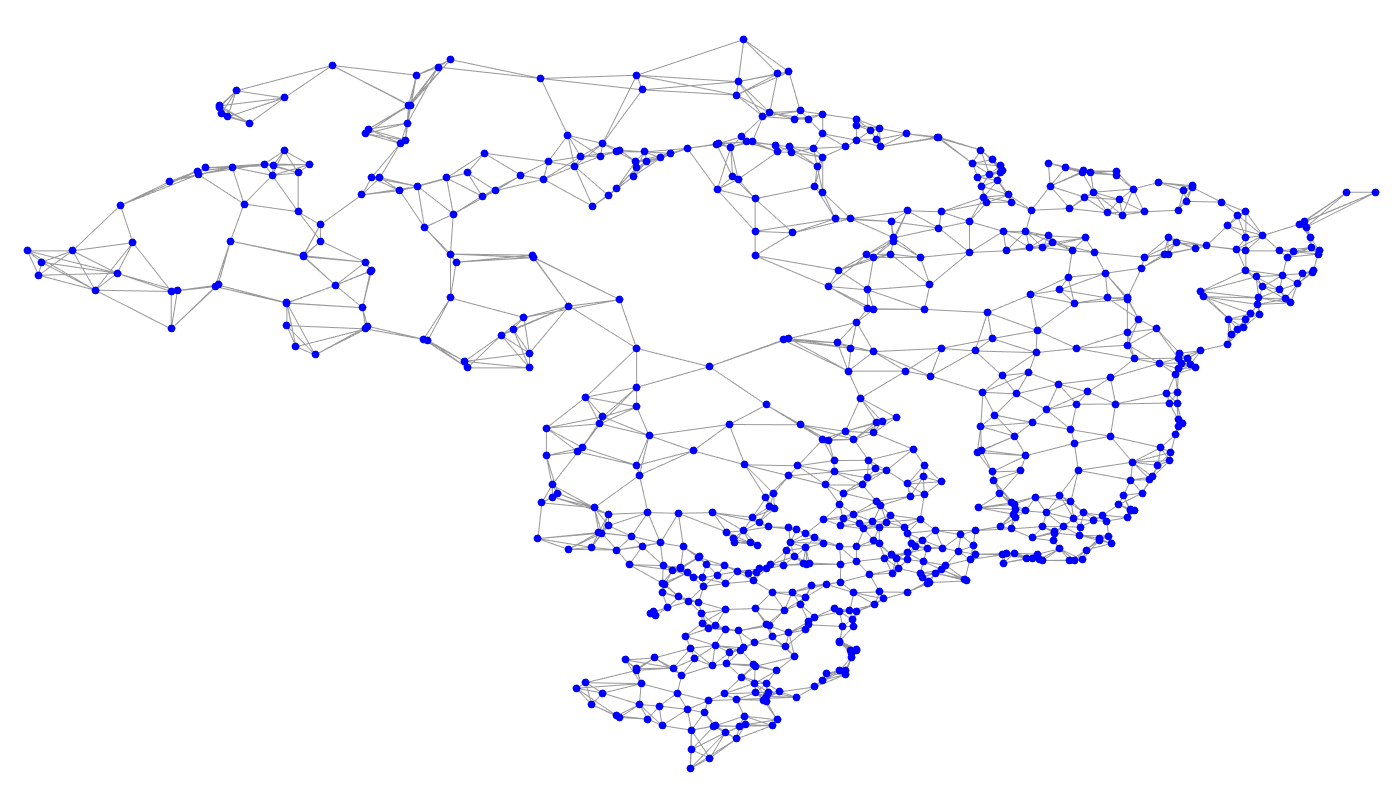
\includegraphics[width=2in, height=2in] {figures/brazil_graph_nn_5.png}
		\label{fig:brazil_graph_nn_5}
	}
	\subfigure[]{
		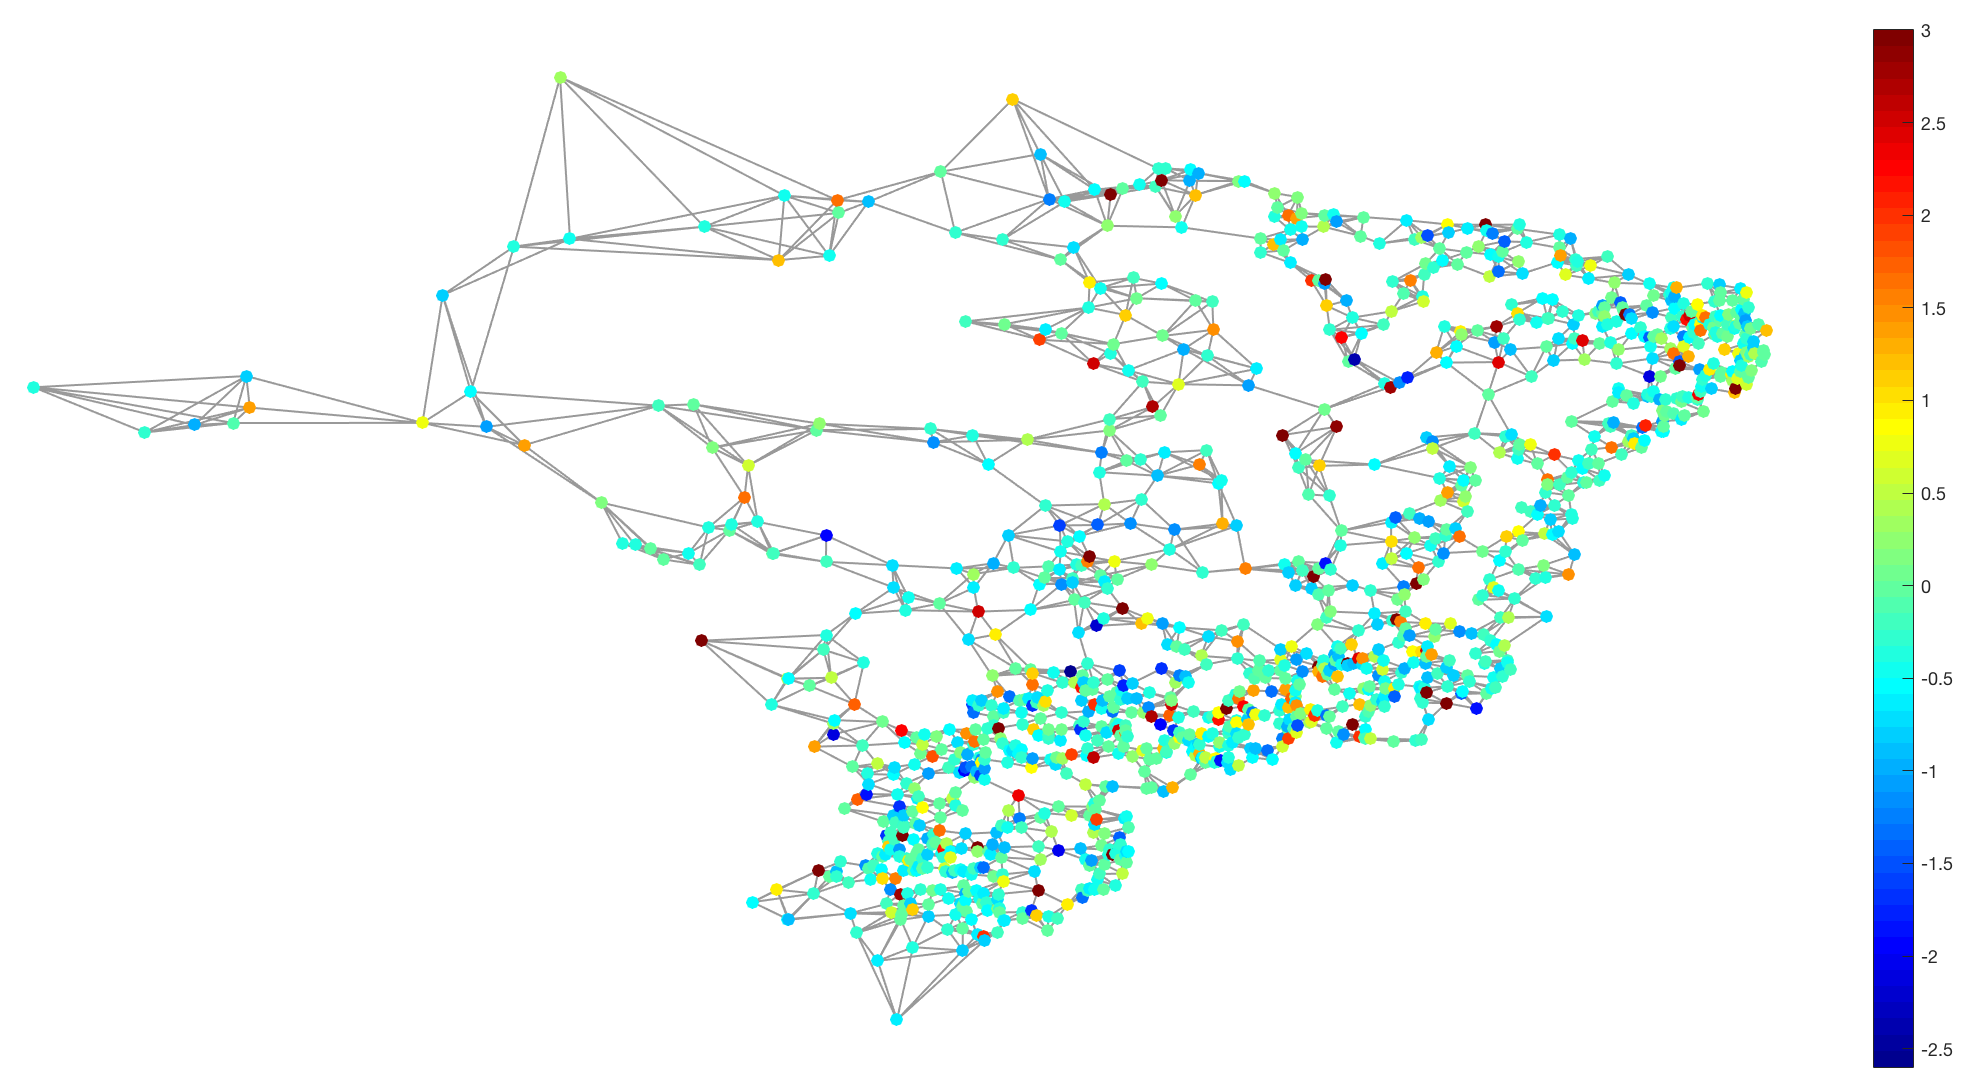
\includegraphics[width=2in, height=2in] {figures/brazil_zscore_31.png}
		\label{fig:brazil_zscore_31}
	}
	\caption{(a) Brazil $5$ nearest-neighbor Graph: 1276 cities an all edge weights are $1$. (b) Brazil $Z_{score}$ on July 31th, 2013, the color bar shows the scale of $Z_{score}$.}
	\label{fig:graphwaveletcoefficient}
\end{figure}


\paragraph{Time Series $Z_{score}$}
Considering the Twitter count $X$ varies vastly among cities,  instead of using $X$ itself, we use the normalized value $Z_{score}$, which is defined as:
\begin{equation}
\label{eq:Z_score}
Z_{score}= \frac{X-\mu}{\sigma}
\end{equation}Where, $\mu$ is the mean value of the previous $30$ days Twitter counts , and $\sigma$ is the corresponding standard deviation. As shown in Figure~\ref{fig:brazil_zscore_31}, different node color shows cities' different $Z_{score}$ value.

\paragraph{kernel function, $g(x)$ and scaling function $h(x)$}
Our choice for the wavelet generating kernel function, $g(x)$ and scaling function $h(x)$ is motivated by our goal to achieve scale-dependent localization. We set $g(x)$ and $h(x)$ as:
\begin{equation}
g(x) = \left\{ \begin{array}{rl}
 x &\mbox{ for $x<1$} \\
s(x) &\mbox{ for $1\leq x \leq 2$} \\
 2x^{-1} &\mbox{ for $x>2$} \\
       \end{array} \right.
\end{equation}, where $s(x)=-5+11x-6x^2+x^3$.
\begin{equation}
h_{x}= 1.385*exp(-(\frac{20x}{0.6\lambda_{max}})^4)
\end{equation}
The scale set $\{s_j\}_{j=1}^J$ is selected to be equally logarithmically spaced between the minimum and maximum scales $s_1$ and $s_J$, which are defined in~\cite{hammond2011wavelets}. We set $J=6$ in the experiments.

\paragraph{anomaly index $\gamma_f(G)$ and $\omega_{th}$}
We claim that the event frequency $\eta$ is linear to $\gamma_f(\mathbf{G})$, and the linear equation is
\begin{equation}
\label{eq:linear_equation}
\eta = k_0*\gamma_f(\mathbf{G}) + k_1
\end{equation}We use historical data for training of $k_0$ and $k_1$ by least square error criterion. Once we know
$k_0$ and $k_1$, given a new $\gamma_f'(\mathbf{G})$, the events number is estimated as $m=\left \lceil \eta' \right \rceil$. After that the threshold $\omega_{th}$ is set as the $m$ largest $W_f(s_j,a)$, for all $a\in V$, $0\le j \le J$.




\begin{table}[bth] %!htp
\renewcommand{\arraystretch}{1.1}
\caption{\label{table:models_compare} The performance of graph wavelet vs. baseline and Zscore.}
\scriptsize
\centering
\begin{tabular}{ l | l |l | l | l}
\hline
\textbf{Country} & \textbf{Method}& \textbf{Precision}  & \textbf{Recall}  & \textbf{F-measure} \\
\hline
Mexico & Baseline & 0.074 &0.124 & 0.090 \\
       & Zscore & 0.221 &0.147 & 0.168 \\
 & Graph wavelet& 0.397 &0.384 & 0.408 \\
\hline
Brazil & Baseline & 0.052 &0.104 & 0.060\\
       & Zscore & 0.117&0.307 & 0.159 \\
 & Graph wavelet& 0.404 &0.262 & 0.292 \\
\hline
Venezuela & Baseline & 0.078 &0.053 & 0.059 \\
       & Zscore & 0.197 &0.197 & 0.189 \\
 & Graph wavelet& 0.292 &0.554 & 0.355 \\
\hline
\end{tabular}
\end{table}



\subsection{Performance}
We did experiment on three major protest countries: Brazil, Mexico and Venezuela, from Jan 2013 to Dec 2014. Taken the Gold Standard Report (GSR) as grand truth, we run the graph wavelet approach. For each day, decide whether there is any anomaly, if there is, identify the group of abnormal cities, then compare with GSR, see if the selected cities have protest events on that day, how many of them are matched with truth, how many of them do not have protest. We use recall, precision and F-measure to evaluate the performance.



\begin{figure}[h]
	\centering
    {
		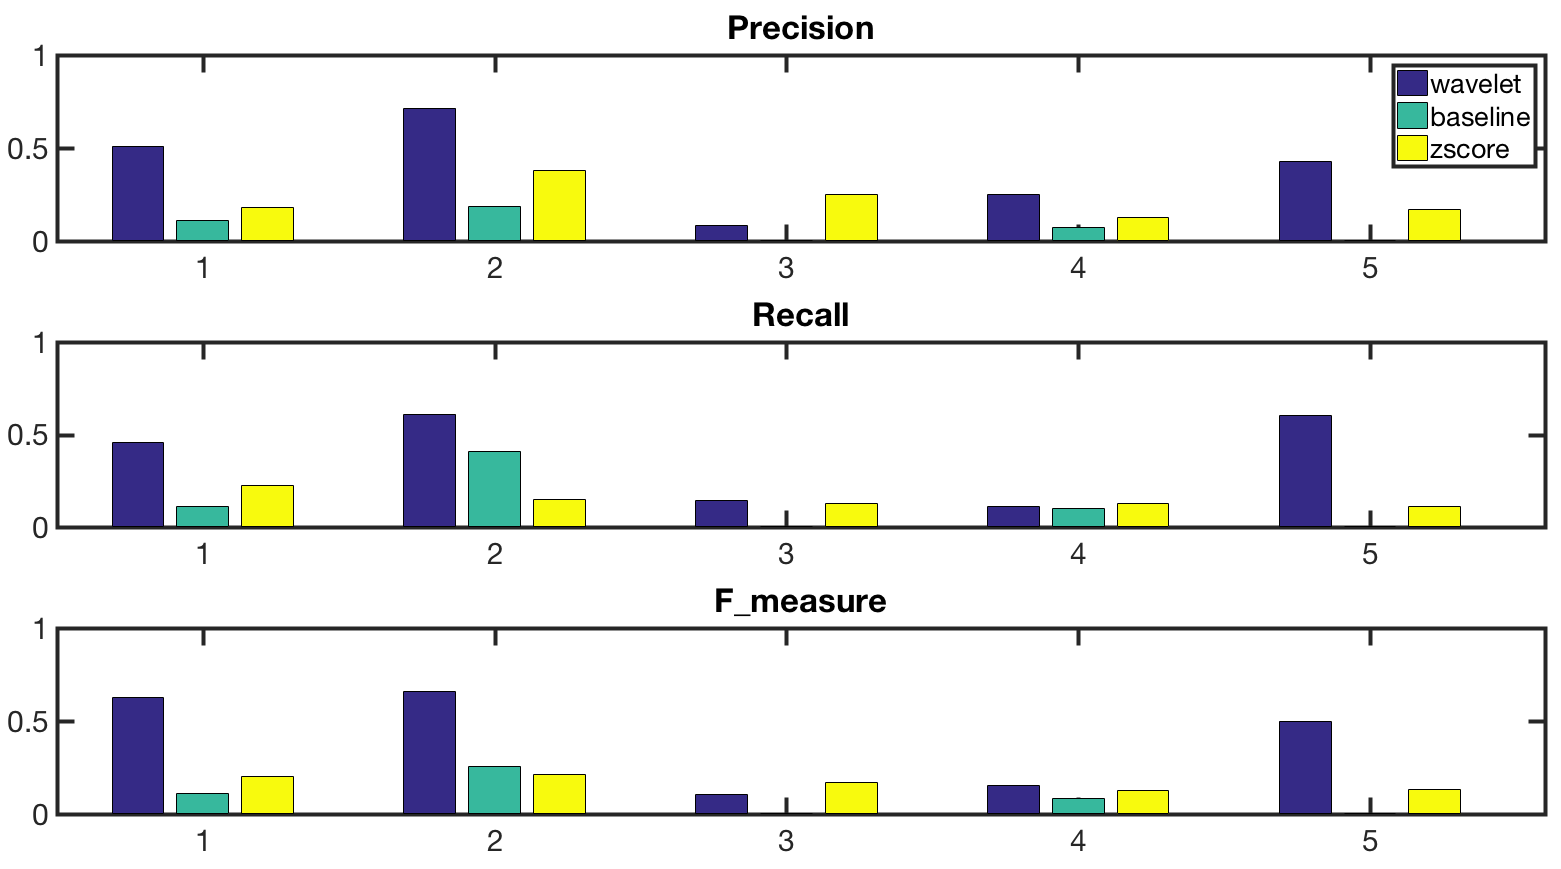
\includegraphics[width= 4in] {figures/performance_compare_bar_graph_mexico.png}
		\label{fig:distribution2}
	}
	\caption{Mexico protest detection performance.}
	\label{Mexico_performance}
\end{figure}



\begin{figure}[h]
	\centering
    {
		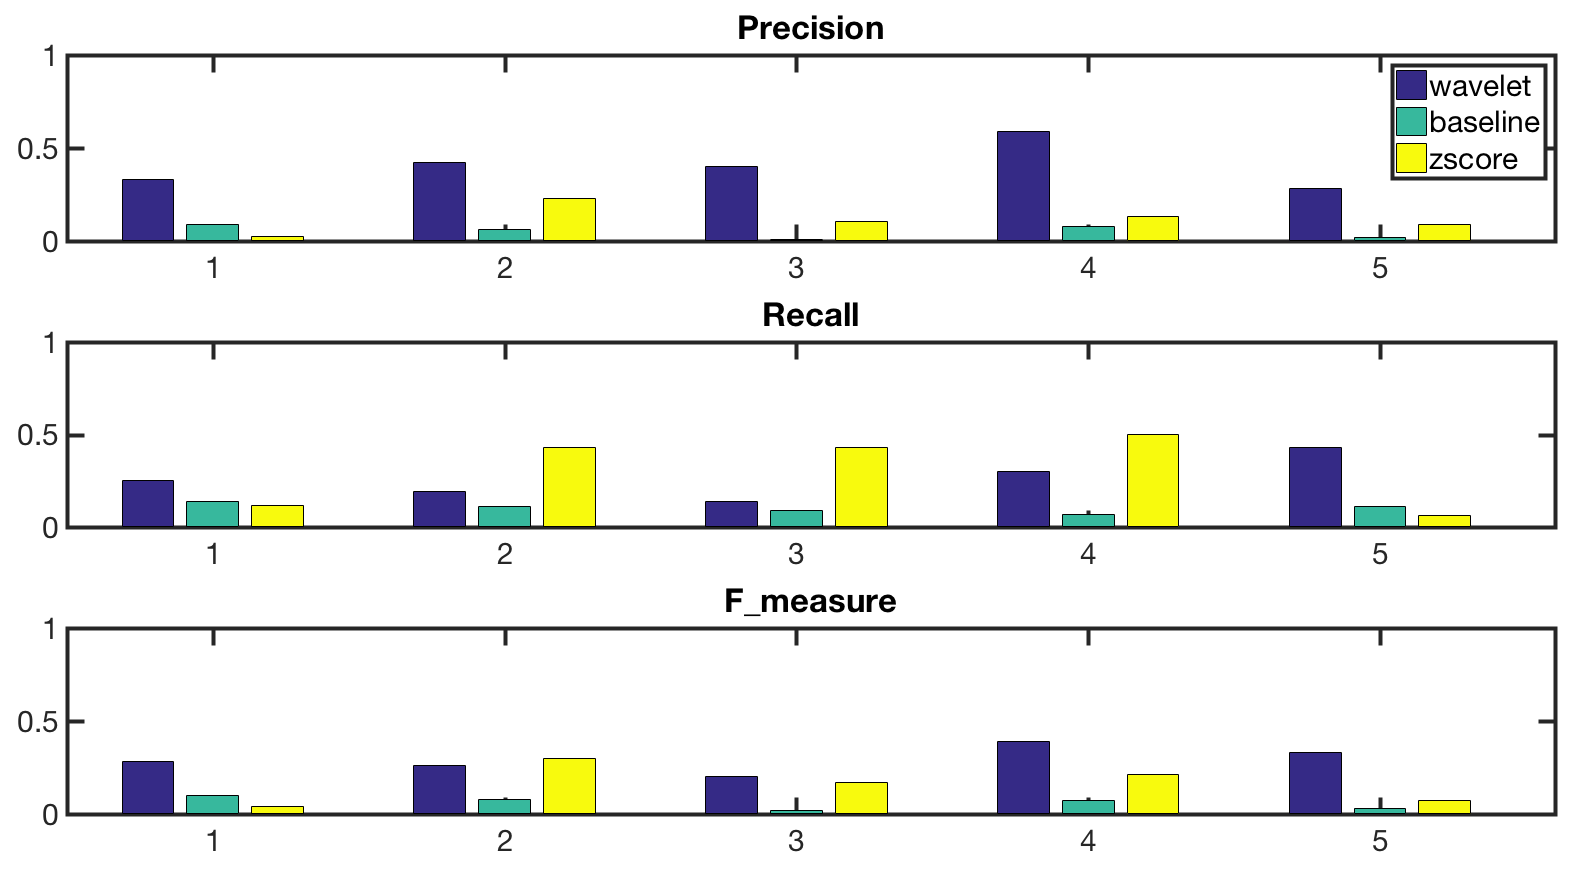
\includegraphics[width= 4in] {figures/performance_compare_bar_graph_brazil.png}
		\label{fig:distribution2}
	}
	\caption{Brazil protest detection performance.}
	\label{Brazil_performance}
\end{figure}


\begin{figure}[h]
	\centering
    {
		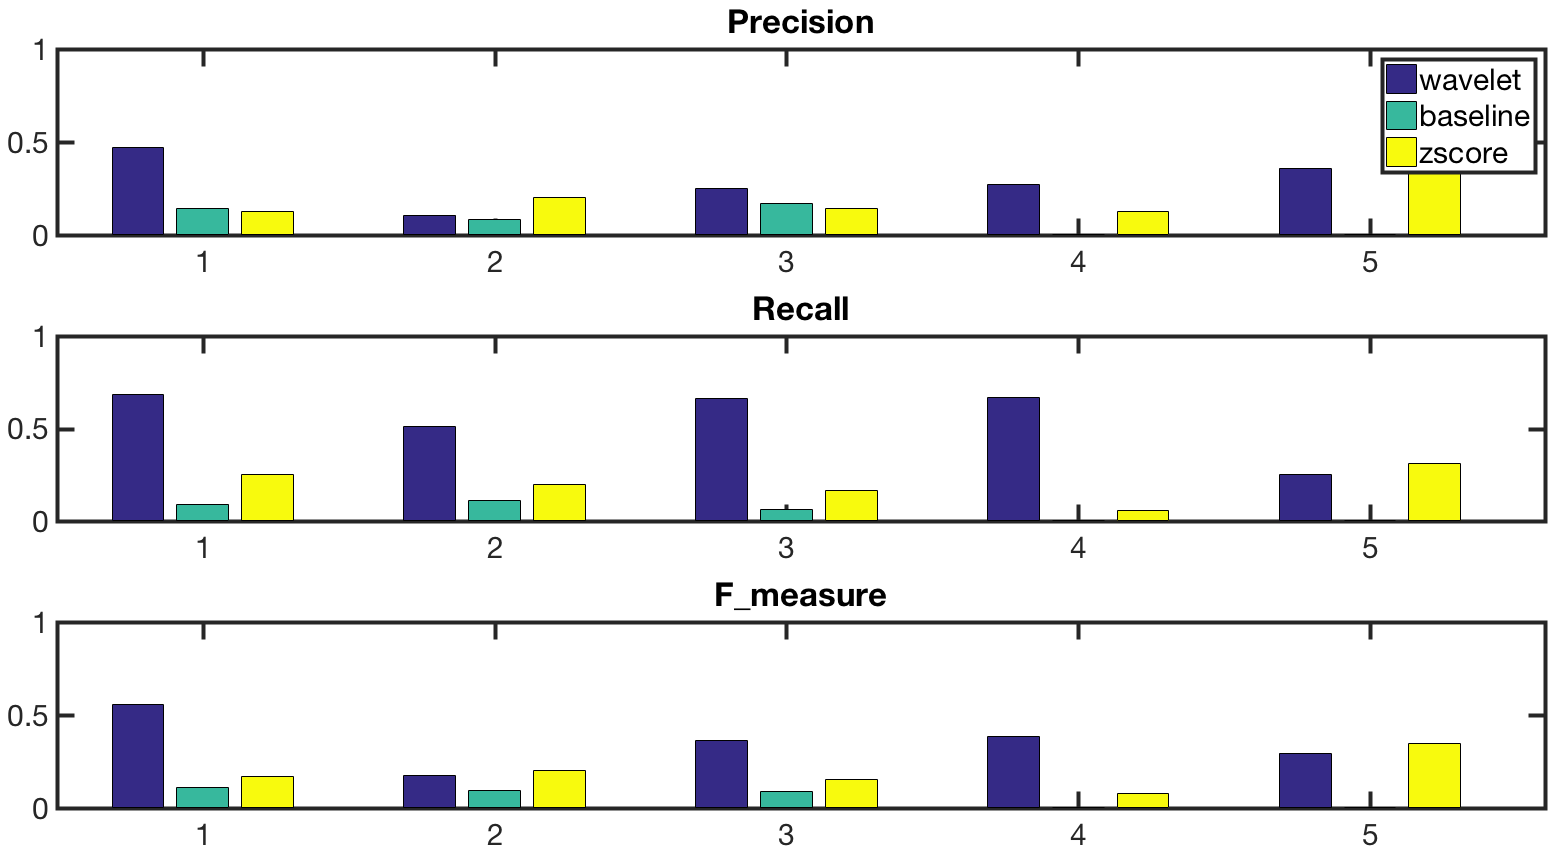
\includegraphics[width= 4in] {figures/performance_compare_bar_graph_venezuela.png}
		\label{fig:distribution2}
	}
	\caption{Venezuela protest detection performance.}
	\label{Venezuela_performance}
\end{figure}


To evaluate our graph wavelet approach, we also compare with some intuitive approaches, like frequency based random assign, we call it baseline model, and Z-score based selection methods. The baseline model is built according to the historical protest records of each city, based on frequency, predict the future protests occurrence. The Z-score approach is, selecting the group of cities whose Z-score across some threshold, say say $|Zscore|>3$.

We compare three models performance over two years period test, and show the overall results on Table~\ref{table:models_compare}. Generally speaking, graph wavelet has better precision, recall, and F-measure scores than baseline across countries. The mean F-measure for graph wavelet detection across models and countries is greater than that for other predictions. Interestingly, we find that the graph wavelet work at different efficiency levels depending on each countries. Compared with Figure~\ref{Brazil_performance}, Figure~\ref{Mexico_performance} and Figure~\ref{Venezuela_performance}, we found graph wavelet model has a much higher recall in Venezuela than in Brazil, while graph wavelet has a inferior quality of event detection in Mexico than in Venezuela.



\subsection{Case Studies}
\label{sec:highlighted_results}

\begin{figure}[t]
	\centering
	\subfigure[]{
		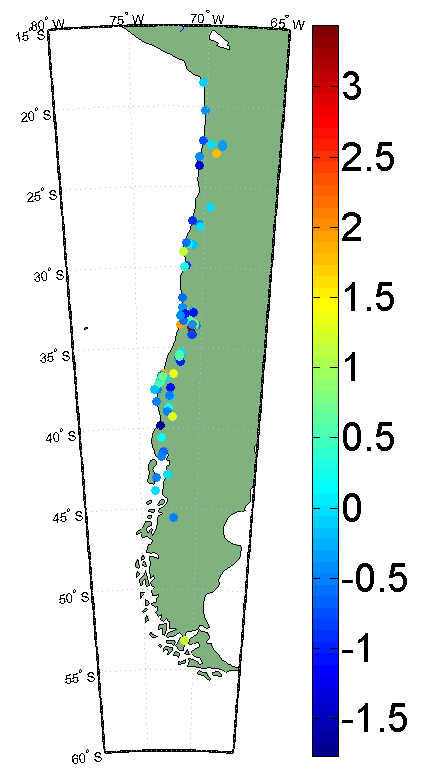
\includegraphics[width=1.3in,height=1.5in] {figures/Chile_absent_zscore_3.png}
		\label{fig:absent_Chile_score}
	}
	\hfill
	\subfigure[]{
		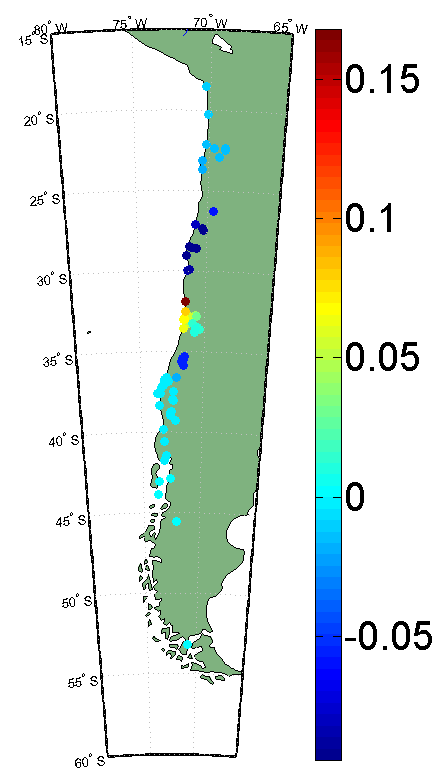
\includegraphics[width=1.3in,height=1.5in] {figures/Chile_absent_wavelet_3.png}
		\label{fig:absent_Chile_wavelet}
	}
	\hfill
	\subfigure[]{
		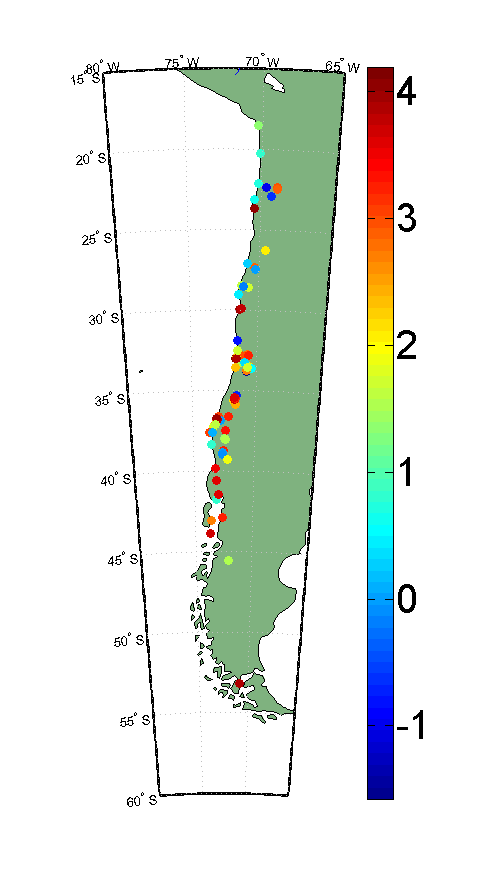
\includegraphics[width=1.3in,height=1.5in] {figures/Chile_burst_zscore_3.png}
		\label{fig:burst_Chile_score}
	}
	\hfill
	\subfigure[]{
		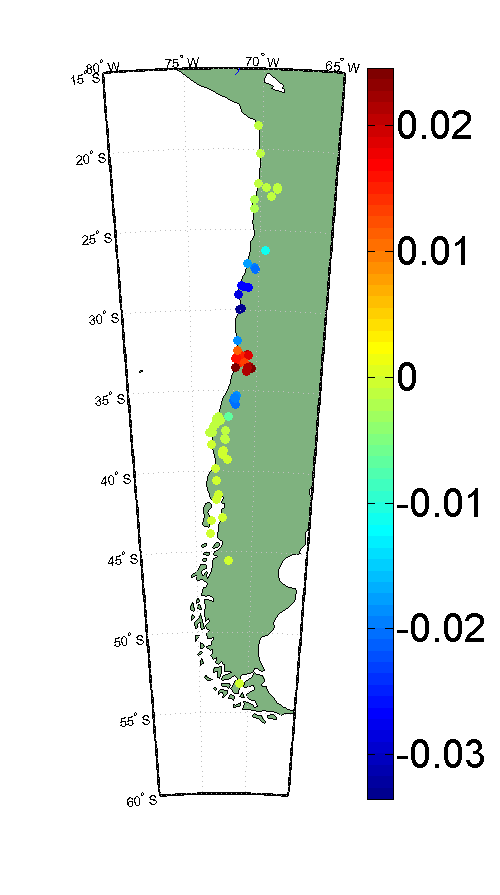
\includegraphics[width=1.3in,height=1.5in] {figures/Chile_burst_wavelet_3.png}
		\label{fig:burst_Chile_wavelet}
	}
\vspace{-2mm}
	\caption{Iquique Earthquake, Chile. Above plots show differences in distributions of absenteeism score and wavelet coefficients calculated at 8:45 PM, April 1, 2014 (a-b) involving group absenteeism and later when burst in activity is captured at 11:00 AM, April 2, 2014 (c-d), respectively.}
\label{fig:case1_wavelet}
\end{figure}

\begin{figure}[t]
	\centering
	\subfigure[]{
		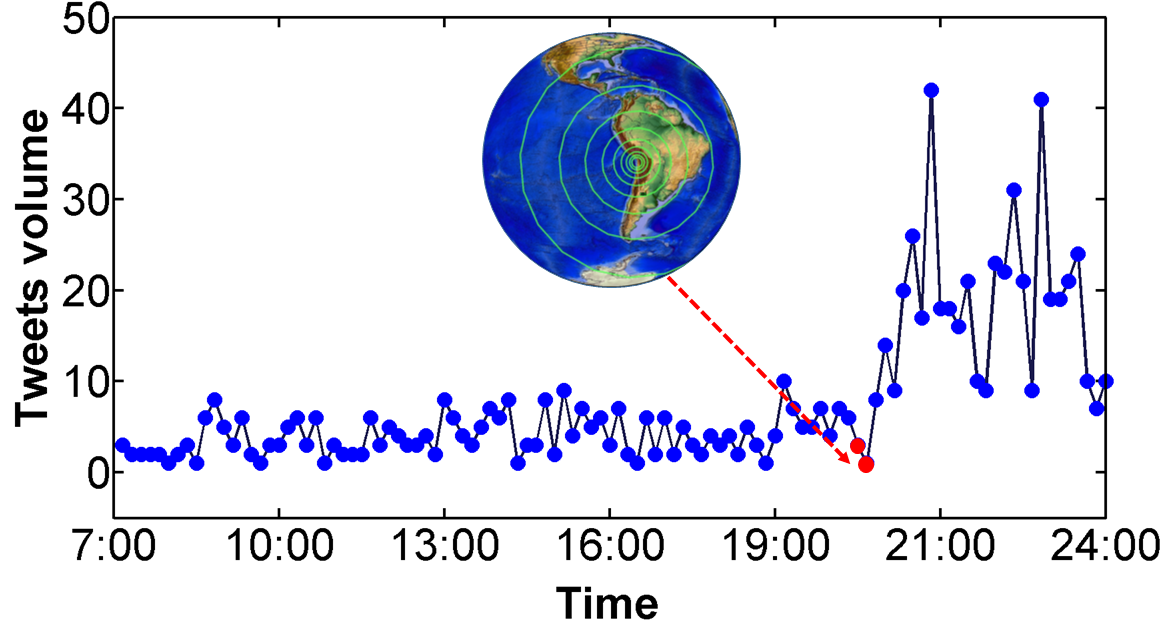
\includegraphics[width=3in,height=1.5in] {figures/earthquake_example_10min_circle.png}
		\label{fig:earthquake}
	}
	\subfigure[]{
		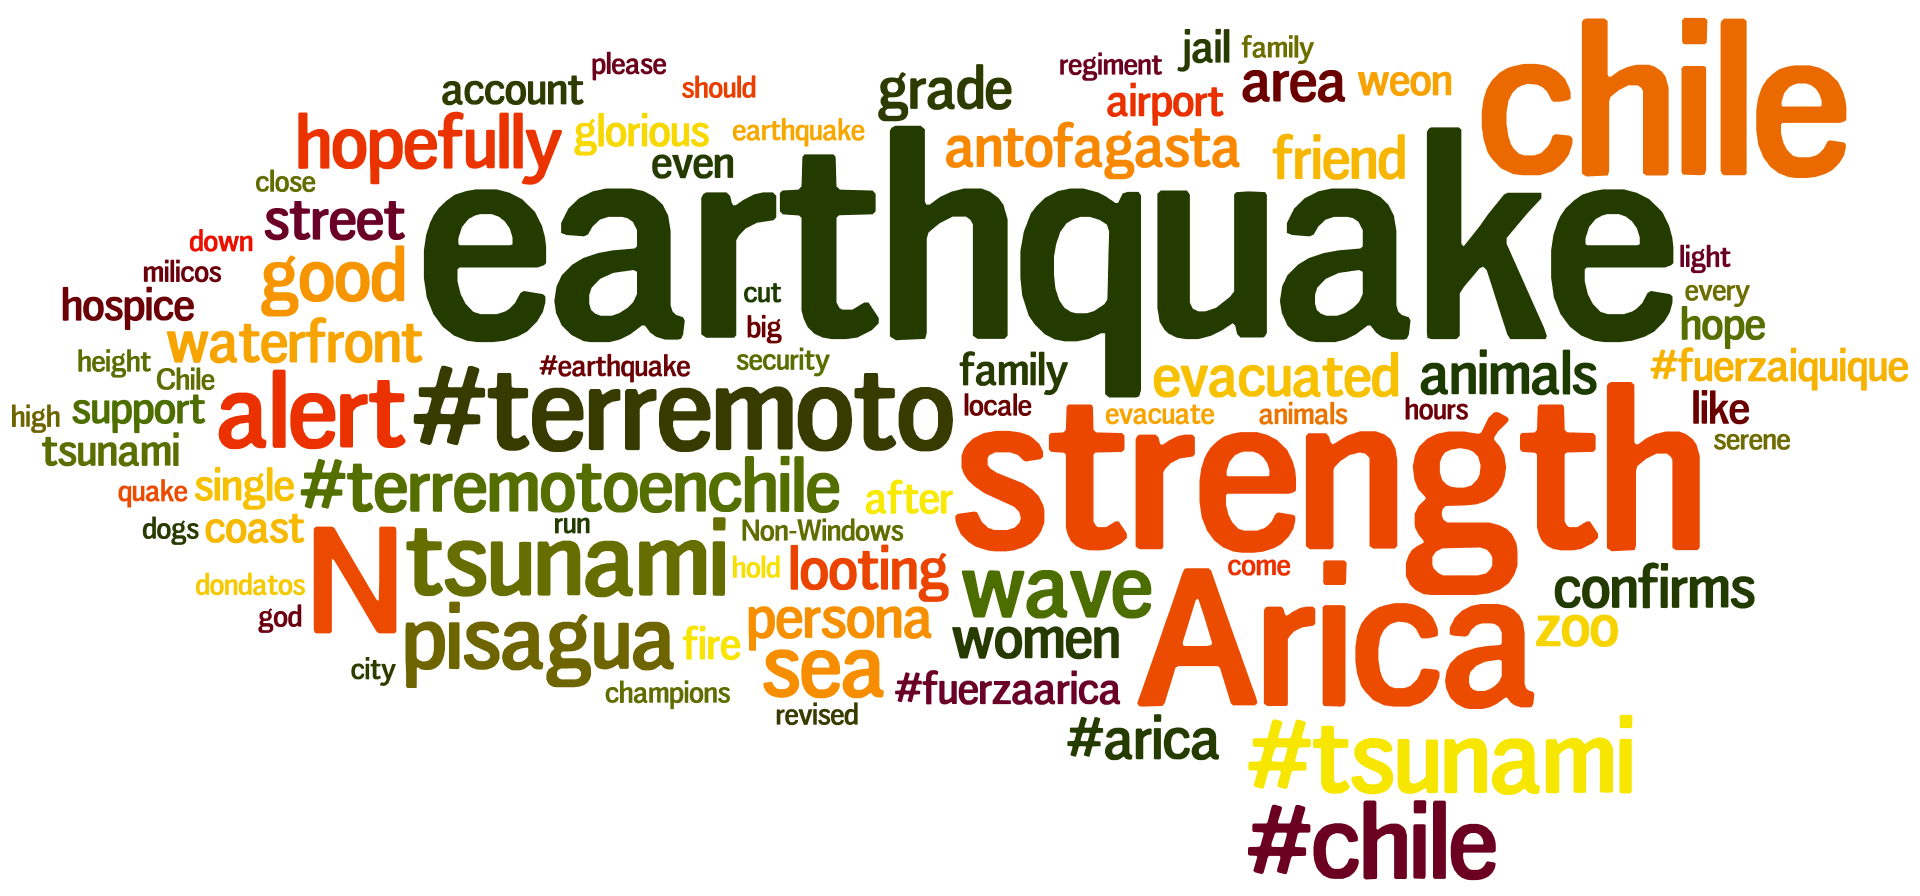
\includegraphics[width=3in,height=1.5in] {figures/earthquake_cloud.png}
		\label{fig:earthquake-cloud}
	}
\vspace{-2mm}	
	\caption{Iquique earthquake, Chile, April 1, 2014. (a) Tweet time series for Iquique on April 1, 2014. (b) Word cloud of tweets which mention `Iquique'.}
\label{fig:case1_cloud}
\end{figure}

\textbf{Case study 1: Iquique Earthquake, Chile.}
On April 1, 2014 around 8:46 PM (local time) a large earthquake struck off the coast of Chile, northwest of the port city of Iquique.
We show the distribution of absenteeism scores and normalized wavelet coefficient values of the graph wavelets from the beginning of this event and over a 24 hour period.
As shown in Figure~\ref{fig:absent_Chile_score} we observe an absenteeism behavior, where the scores are dominated by very low (blue spectrum) of Z-score values (indicating high absenteeism).
Likewise in Figure~\ref{fig:absent_Chile_wavelet}, we witness low coefficients values for the northern regions of Chile, where the impact of the earthquake was most significant.
As the news of earthquake spread throughout the next day, user activity on social media increased. This bursty behavior is seen on April 2nd, around 11:00 AM. We can observe from Figure~\ref{fig:burst_Chile_score} that our z-scores have increased (red spectrum) significantly and the coefficient value distribution (see figure~\ref{fig:burst_Chile_wavelet}) of graph wavelets, for northern regions of Chile is now in red spectrum.
From the graph wavelet distributions in Figs. ~\ref{fig:absent_Chile_wavelet}~\ref{fig:burst_Chile_wavelet}, we can see that the kernel area of the absenteeism/burst wavelets cover most large negative/positive values.
In this way, the wavelet identifies the abnormal negative/positive groups in absent/burst time intervals, respectively.
Furthermore, a high correlation score of 0.726 was calculated for the wavelets from absenteeism and bursty periods of this episode.
As a result, we note that there is a strong connection between the burst in activity and the previously observed absenteeism, signaling an event was detected.


From the graph wavelets generated in absenteeism time period~\ref{fig:absent_Chile_wavelet}, we found the central node to be the city of `Iquique'.
We study the timeseries (Fig.~\ref{fig:earthquake}) of Twitter activity for Iquique and word clouds (see Fig..~\ref{fig:earthquake-cloud}) generated from their content, to see how events unfolded during the course of the earthquake.
Strong absenteeism is observed from 8:45 PM to 9:20 PM. We also checked  user mobility through geotagged tweets from city of Iquique, on April 1, 2014 and found that the user mobility fraction had increased by 15.4\%.

\begin{figure}[t]
	\centering
	\subfigure[]{
		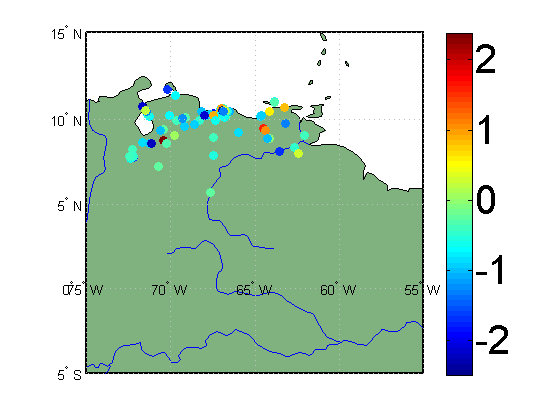
\includegraphics[width=1.4in, height=1.4in] {figures/Venuze_absent_zscore_3.png}
		\label{fig:absent_Venezuela_score}
	}
	\subfigure[]{
		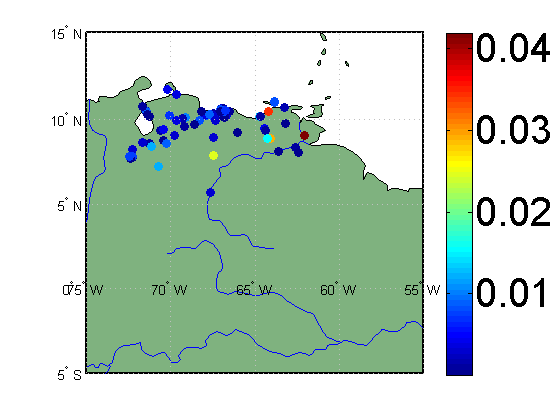
\includegraphics[width=1.4in,height=1.4in] {figures/Venuze_absent_wavelet_3.png}
		\label{fig:absent_Venezuela_wavelet}
	}
	\subfigure[]{
		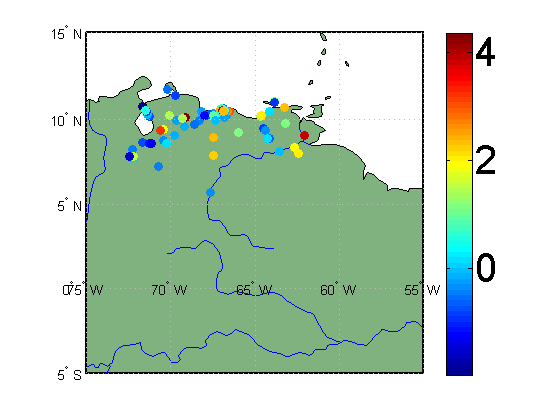
\includegraphics[width=1.4in,height=1.4in] {figures/Venuze_burst_zscore_3.png}
		\label{fig:burst_Venezuela_score}
	}
	\subfigure[]{
		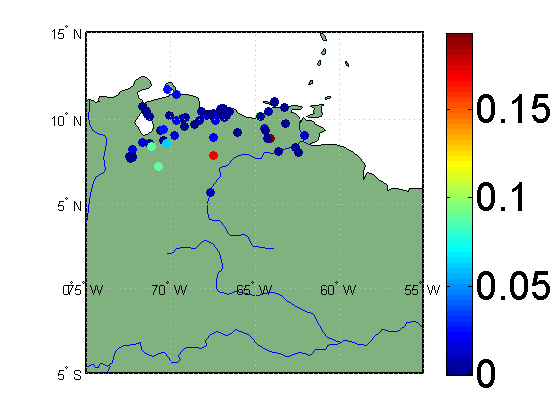
\includegraphics[width=1.4in,height=1.4in] {figures/Venuze_burst_wavelet_3.png}
		\label{fig:burst_Venezuela_wavelet}
	}
    \vspace{-2mm}
	\caption{Power Outage in Venezuela. Above plots show differences in distributions of absenteeism score and wavelet coefficients calculated at 7:40 PM, December 2, 2013 (a-b) involving group absenteeism and later when burst in activity is captured at 8:45 PM in the same day (c-d), respectively.}
\label{fig:case2_wavelet}
\end{figure}


\begin{figure}[th]
	\centering
	\subfigure[]{
		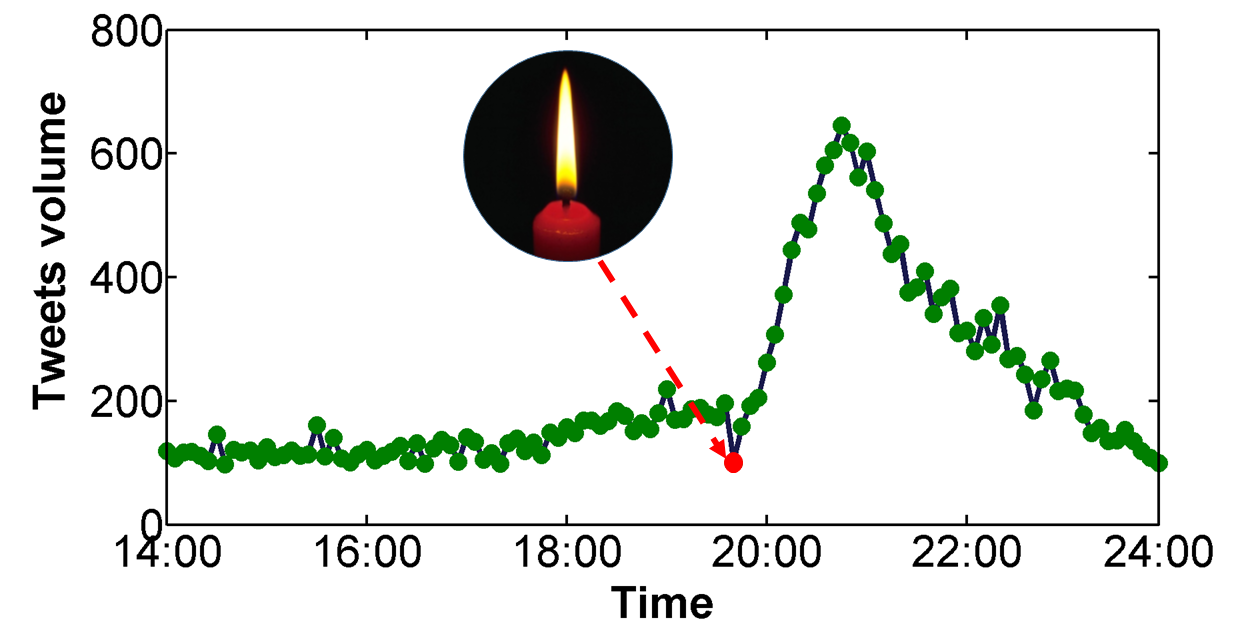
\includegraphics[width=3in,height=1.5in] {figures/Veneuela_power_count_all.png}
		\label{fig:power}
	}
	\subfigure[]{
		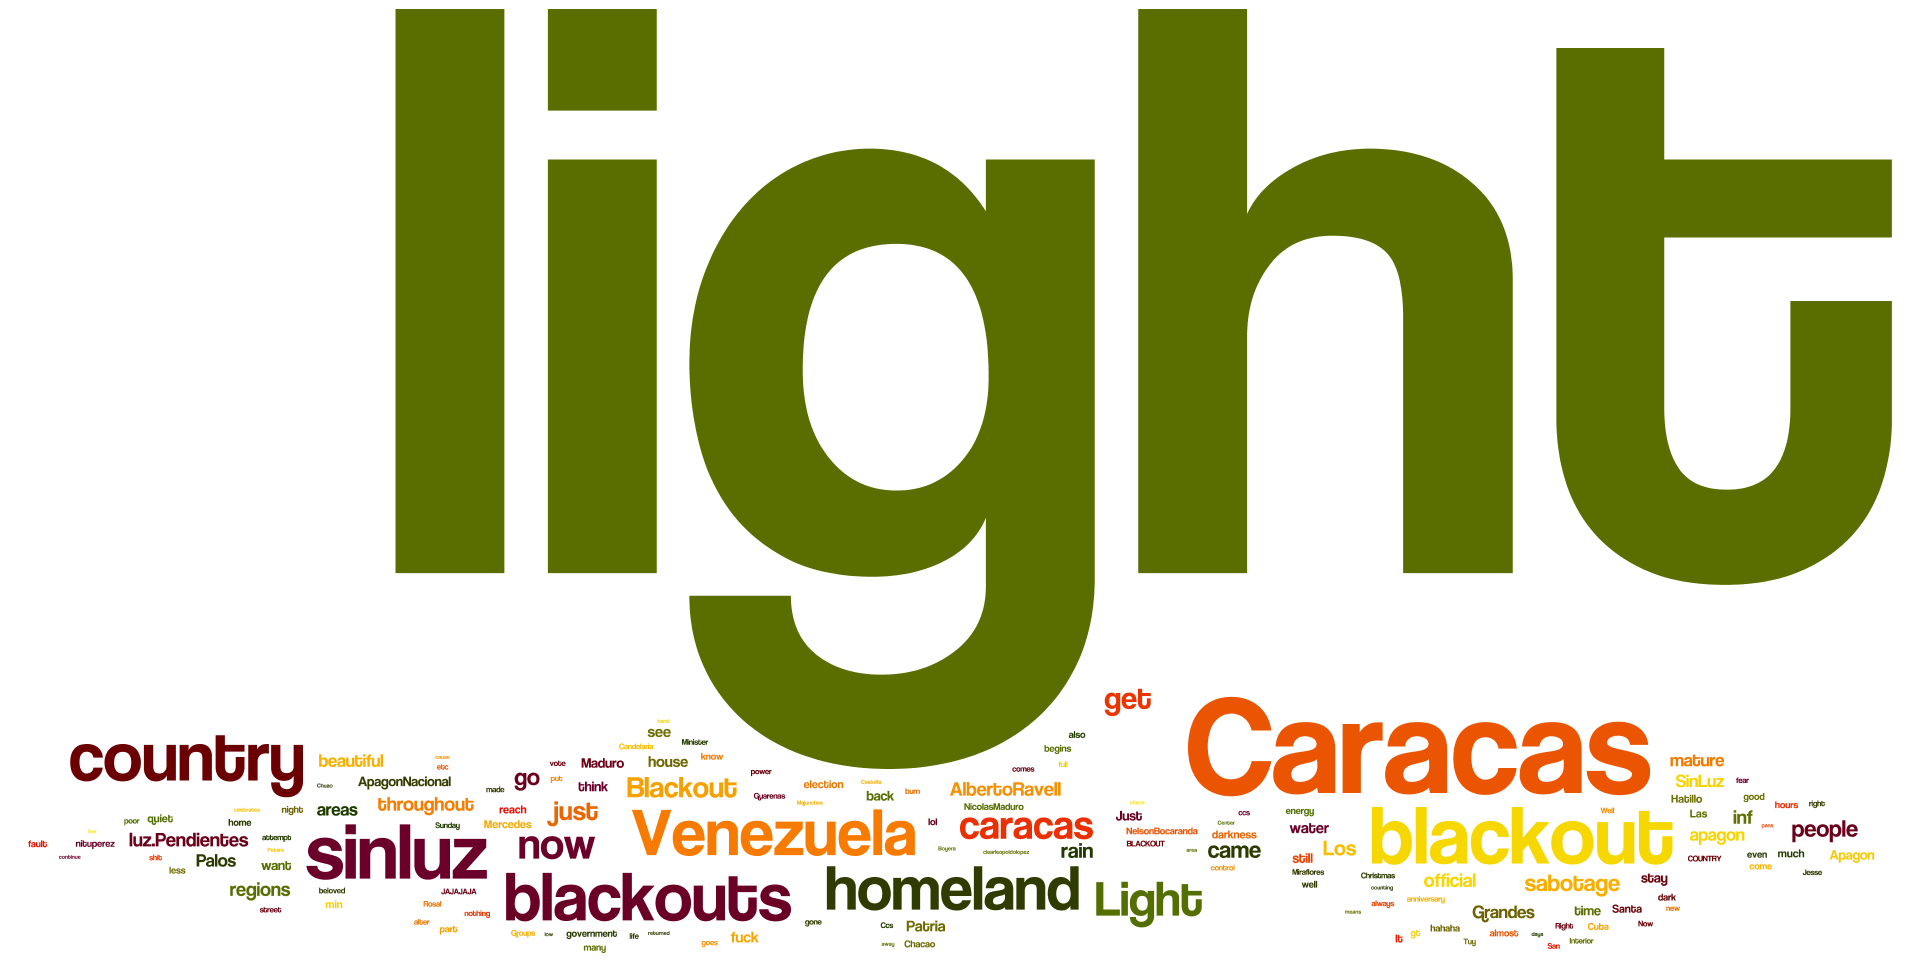
\includegraphics[width=3in,height=1.5in] {figures/power-English.png}
		\label{fig:power-cloud}
	}
    \vspace{-2mm}
	\caption{Caracas, Venezuela power outage, December 2, 2013. (a) Time series of tweets volume. (b) Word cloud of tweets mentioning `Caracas'.}
\label{fig:case2}
\end{figure}


\textbf{Case Study 2: Massive power outage in Venezuela.}
A massive power outage in Venezuela plunged several major cities including the capital city, Caracas in to darkness around 7:40 PM (local time) on December 2, 2013.
News media reported~\footnote{http://www.usatoday.com/story/news/world/2013/12/\hskip0ex 02/\hskip0ex power-failure-caracas-venezuela/3823327/}, that the power outage lasted for 10-15 minutes, and the people of Caracas soon went out in the streets to protest.
This action at the beginning of the episode coincides with the absenteeism period detected by our algorithm.
The scatter plots showing distribution of absenteeism scores and wavelet coefficients (Figs.~\ref{fig:absent_Venezuela_score},~\ref{fig:absent_Venezuela_wavelet}) indicate that most of the low values are less than $0$.
Shortly after the absenteeism, we detected a huge burst in activity around 8:45 PM, signaled by the increased z-scores (low absenteeism) and coefficient values (Figs.~\ref{fig:burst_Venezuela_score},~\ref{fig:burst_Venezuela_wavelet}).
A correlation score of 0.617 was calculated on comparing the graph wavelets from both absentee and burst period.

The absenteeism related graph wavelets indicated that the city of Caracas
%`San Fernando de Apure'
was the central node. Taking a close look at the twitter volume and tweets from Caracas and surrounding cities, we observed a sharp decline in user activity right around 7:40 PM and then a huge spike at starting at 8:45 PM.
The word clouds of tweet content show a very similar story.
The most dominant words are `light' and `blackout', even the Spanish phrase `sin luz' which means `no light' became a trending hashtag \#sinluz on Twitter.


\textbf{Case Study 3: Christmas Day.}
As mentioned earlier, an absenteeism behavior may not always lead to a spike in activity. In this case, our model detected strong absenteeism in social media activity for major holidays such as Christmas day, however it was not followed by a bursty period in Twitter activity. One explanation of this behavior is that people tend to travel back to visit family during the holidays. This is supported by low values of z-scores or high absenteeism in Figure~ \ref{fig:absent_Argentina_score} and wavelet coefficients in Figure~\ref{fig:absent_Argentina_wavelet} with respect to Argentinian tweets on December 25, 2013. Hence, no subsequent burst period was detected for this event.

\begin{figure}[t]
	\centering
	\subfigure[]{
		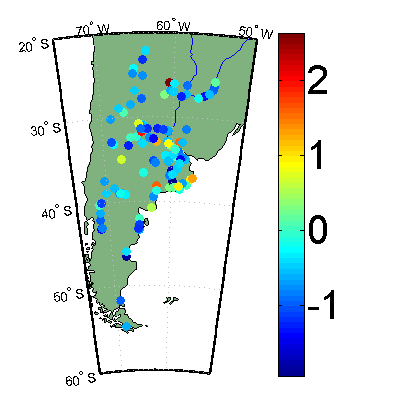
\includegraphics[height=1.5in] {figures/Argentina_absent_zscore_3.png}
		\label{fig:absent_Argentina_score}
	}
	\subfigure[]{
		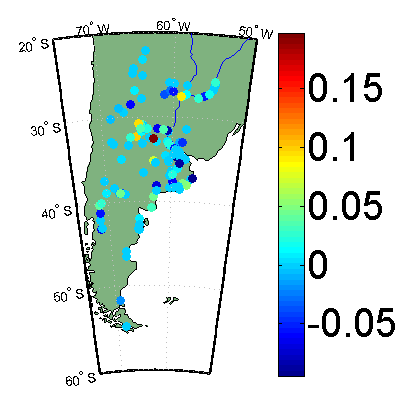
\includegraphics[height=1.5in] {figures/Argentina_absent_wavelet_3.png}
		\label{fig:absent_Argentina_wavelet}
	}
	\subfigure[]{
		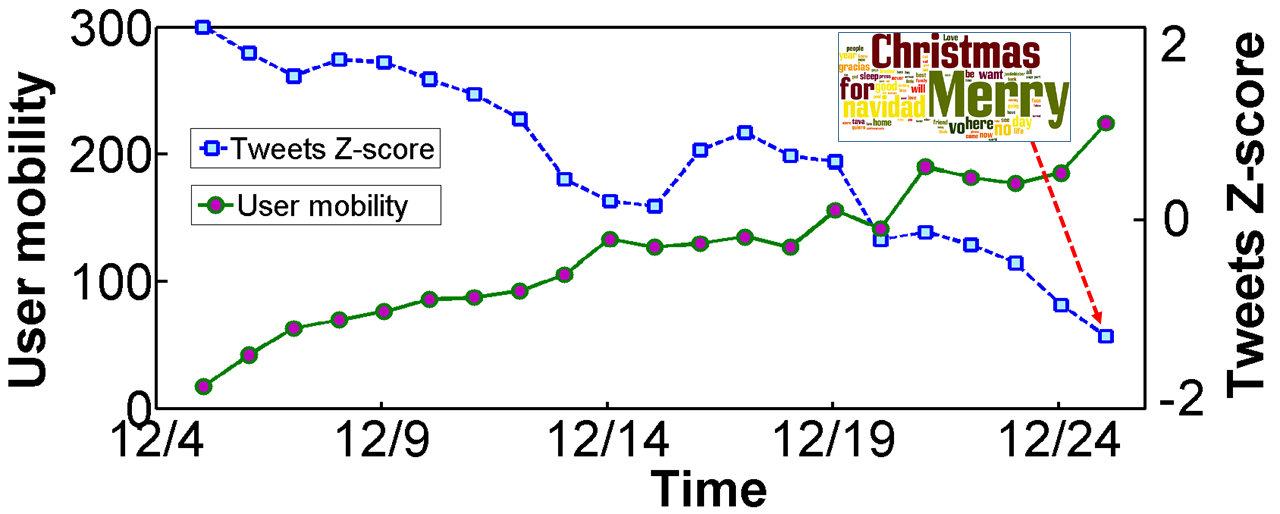
\includegraphics[width=2.7in,height=1.4in] {figures/holiday-cloud.png}
		\label{fig:holiday-cloud}
	}
	\caption{The Christmas Day in Argentina: Above plots shows distributions of (a) absenteeism score and (b) wavelet coefficients calculated on December 25, 2013. (c) Time series comparing absenteeism score and user mobility corresponding to tweets between December 5, 2013 and December 25, 2013.}
\vspace{-2mm}
\label{fig:case3_wavelet}
\end{figure}



Interestingly as the Christmas day approached we observed (see Figure~\ref{fig:holiday-cloud}) that user mobility gradually increases and z-score decreases signaling greater absenteeism. We used Pearson's correlation coefficient to measure the two time series and found a correlation score of -0.94.
\subsection{Why Absenteeism Group Detection?}
Previous research has demonstrated the importance of burst detection in Twitter. In our study, we argue that group absenteeism can also be vital for detecting disruptive societal events. Modeling absenteeism is crucial, because it can serve as a surrogate signal for event detection. For example, in the case of the Iquique earthquake, where our algorithm  detected an absenteeism behavior on Twitter followed by a spike in user activity. Unlike traditional event detection methods which identify real time events only after they have occurred i.e., once the burst signal has been identified; the absenteeism signal can be observed much earlier, and it renders a foresight or view into the future events. Our approach thus offers a significant advantage over current strategies that focus solely on modeling spike or burst related patterns for event detection.

%Disruptive events which cause Twitter absenteeism, but also render burst detection methods less useful. In the case of the Natal protest event, a large portion of people were walking on the street to protest, and the city's tweet absenteeism score reached a minimum. During the Brazil floods, the tweets tended to become inactive as the severity of the floods increased. It reached the lowest point when the flood was at its worst. In these two cases in particular, using a burst signal alone it can be difficult to identify such events.


%%%%%%%%%%%%%%%%%%%%%%%%%%%% end %%%%%%%%%%%%%%%%%%%%%%%%%
%\begin{table*}[th] %!htp
% \renewcommand{\arraystretch}{1}
% \caption{\label{table:list_events} Selected major events in South America countries}
% \scriptsize
% \centering
% \begin{tabular}{ p{0.5cm}| p{2cm} | p{2.2cm} | p{2.2cm} | p{2.2cm} | p{2.5cm} | p{3cm} }
%  \hline
%  \textbf{No.} & \textbf{Events}& \textbf{ Absenteeism } & \textbf{Response time} & \textbf{Correlation}&\textbf{Central location} \\ [1ex]
%  \hline
%        1& Earthquake & 8:45 PM & 3 hours & 0.73 &Iquique, Chile\\
%        2& Blackout & 7:40 PM & 1 hour & 0.81& Caracas, Venezuela \\
%        3& holiday & one day & 2 days & 0.33 & \\        \hline
% \end{tabular}
%\end{table*}


%Public holidays are typical events causing group absenteeism. One of the most dominant reason is, during public holidays, especially long-time holiday, people tend to travel, which resulting in a high level of local user mobility, and users' mobility will cause Twitter absenteeism accordingly.
%We calculating more cases Pearson's correlation, and plot their distribution in Figure~\ref{fig:pearson}, of which the median value of correlation score is -0.88, and the average correlation score is -0.79. We can see the user mobility plays a forceful role in influencing Twitter absenteeism.

%\subsection{Performance}
%We use the data set on February 27, 2014, and set the time window as one day. We plot the comparison results from two aspects:  running time complexity, and parameter sensibility in figure~\ref{fig:performance},~\ref{fig:running_time},~\ref{fig:sensibility}.
%\begin{figure}[ht]
%	\centering
%	\subfigure[matrix]{
%		\includegraphics[width=1.55in,height=1in] {figures/performance1.png}
%		\label{fig:performance1}
%	}
%	\subfigure[graph]{
%		\includegraphics[width=1.55in,height=1in] {figures/performance2.png}
%		\label{fig:performance2}
%	}
%	\caption{running time vs input parameter.}
%	\label{fig:performance}
%\end{figure}
%\paragraph{Running time}From Figure~\ref{fig:performance}, we can see that the running time of minimal matrix approach increases extremely fast when $A$ is larger than 0.09. While in graph wavelet approach, the increasing speed is much stable as $d_{th}$ increases. This is because minimal matrix approach's time complexity is in proportion to $A^2$, while graph wavelet approach's time complexity is proportional to $d_{th}$. From Figure~\ref{fig:running_time}, we can see clearly that for the minimal matrix algorithm, the running time complexity also increase sharply with the input size $n$, while in graph wavelet approach, the increase speed is moderate. This is because the minimal matrix approach's timing complexity is $O(N^3)$, while graph wavelet approach's time complexity is $O(N^2)$. Thus, the graph wavelet approach is better  than minimal matrix approach in term of running time for a larger absenteeism group.
%\begin{figure}[h]
%	\centering
%	\subfigure[matrix]{
%		\includegraphics[width=1.55in,height=1in] {figures/running_time1.png}
%		\label{fig:running1}
%	}
%	\subfigure[graph]{
%		\includegraphics[width=1.55in,height=1in] {figures/running_time2.png}
%		\label{fig:running2}
%	}
%	\caption{Running time vs input size.}
%	\label{fig:running_time}
%\end{figure}
%\paragraph{Parameter sensibility}In minimal matrix approach, set the input parameter as $A$, and the optimal absenteeism group as $P_{min}$. When $A$ is changed to $A$', the optimal absenteeism group is changed to $P_{min}$, define the output error as the city number that exists in $P_{min}$ but not in $P_{min}'$, and denoted as $P_{min}-P_{min}'$. We define the parameter sensibility as: $$sensibility=\frac{{|P_{min}-P_{min}'|}/{|P_{min}|}}{|A-A'|/{A}}.$$ We plot the minimal matrix approach and graph wavelet approach's sensibility in Figure~\ref{fig:sensibility}. In the minimal matrix approach, when the input parameter error is smaller than 20\%, the output absenteeism group error is less than 5\%. While in the graph wavelet approach, the output absenteeism group error is linear to the input error parameter. This is probably because minimal matrix approach aggregates all the absenteeism score covered by the region, and usually has a much larger city number than the graph wavelet approach, and makes minimal matrix approach better at anti-noise.  All in all, the minimal matrix algorithm focuses on all the cities in the cover group, and has a better global performance at anti-noise, while is inferior to the graph wavelet counterpart in term of running time complexity.
%\begin{figure}[h]
%	\centering
%	\subfigure[matrix]{
%		\includegraphics[width=1.55in,height=1in] {figures/sensibility1.png}
%		\label{fig:sensibility1}
%	}
%	\subfigure[graph]{
%		\includegraphics[width=1.55in,height=1in] {figures/sensibility2.png}
%		\label{fig:sensibility2}
%	}
%	\caption{Sensibility comparison of the two algorithms.}
%	\label{fig:sensibility}
%\end{figure}




% % % % % % % % % % % % % the end% % % % % % % %
%
%\begin{figure}[ht]
%	\centering
%	\subfigure[]{
%		\includegraphics[width=1.55in,height=1in] {figures/Curitiba-Brazil1-cloud.png}
%		\label{fig:holiday}
%	}
%	\subfigure[]{
%		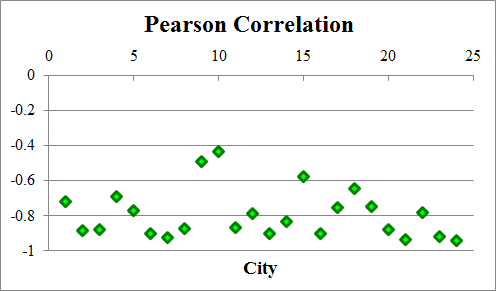
\includegraphics[width=1.55in,height=1in] {figures/pearson1.png}
%		\label{fig:pearson}
%	}
%	\caption{(a) User mobility time series and corresponding absenteeism score, from Dec 5, 2013 to Dec 25, 2013. (b) Pearson correlation score distribution of user mobility and absenteeism score.}
%\label{fig:case3}
%\end{figure}

%Now we show experimental results of our algorithm on highlighted case studies (see Table~\ref{table:list_events}):
%
%\begin{table*}[th] %!htp
%	\renewcommand{\arraystretch}{1}
%	\caption{\label{table:list_events} Selected major events in South America countries}
%	\scriptsize
%	\centering
%	\begin{tabular}{ p{0.5cm}| p{1.5cm} | p{8cm} | p{1.5cm}}
%		\hline
%		\textbf{No.} & \textbf{Date}& \textbf{ Events} & \textbf{Test Areas}   \\ [1ex]
%		\hline
%        1& 2013-06-17 & Brazilian Spring: Protests in over 100 cities, over 2 million people & Brazil  \\		
%        2& 2013-12-02 & Power cut leaves much of Venezuela without electricity & Venezuela \\
%        3& 2013-12-24 & Floods, more than 50,000 people are forced to flee their homes & Brazil\\
%        4& 2013-12-25 & Christmas holiday  & Argentina \\
%        5& 2013-12-30 & Power supply disrupted in heatwave in Buenos Aires, Argentina & Argentina \\
%        6& 2014-04-01 &  M8.2 earthquake struck off the coast of Chile, epicenter is Iquique & Chile  \\
%        7 & 2014-05-21 & Bus strike paralyzes Brazil's biggest city as World Cup looms & Brazil \\			\hline
%	\end{tabular}
%\end{table*}


%The wavelet scales $t_j$ are selected to be logarithmically equispaced between the minimum and maximum scales $t_J$ and $t_1$, with the upper bound $\lambda_{max}$ of the spectrum of $L$. The placement of the maximum scales $t_1$ as well as the scaling function kernel $h$ will be determined by the selection of $\lambda_{min}=\frac{\lambda_{min}}{K}$, where $K$ is a design parameter of the transformation. We then set $t_1$ so that $g(t_1x)$ has power-law decay for $x>\lambda_{min}$, and set $t_J$ so that $g(t_Jx)$ provides monotonicity of the polynomial for $x < \lambda_{max}$. This is achieved by $t_1=\frac{x_2}{\lambda_{min}}$, and $t_J=\frac{x_2}{\lambda_{max}}$. For the scaling function kernel we take $h(x)=\gamma exp(-({{\frac{x}{\lambda_{min}}}})^4)$, where $\gamma$ is set such that $h(0)$ has the same value as the maximum value of $g$.
%
%At each time point the graph has an Z-score vector $f$ and when we get the lowest value for function $< \psi_{t,n},f>$ the corresponding wavelet $\psi_{t,n}$ is reported as an absenteeism pattern.



\section{Conclusion}
\label{sec:conclusion}
Existing approaches for event detection suffer from an inherent latency in their detection process. It is because they use the bursty signals from abnormal activity on social networks, but miss the absenteeism signal that precedes these bursts. Our approach bridges this shortcoming by successfully modeling this \textit{lull-ness}. We have presented a systematic and unified framework for detecting, identifying event's location and distinguishing anomalous groups in Twitter. From the three case studies, we have shown that the initial phase in the evolution of an disruptive, event is characterized by group absenteeism behavior. This behavior is further underlined by an increase in user mobility. As in the case of ``Christmas Day" event we observed absenteeism from Argentina Twitter users in days leading to December 25th was characterized by increased mobility (inferred from geolocated tweets). We defined an absenteeism score over the groups of cities that form our Twitter network and used it construct wavelet transforms, that not only to detect the anomalous subgraphs at different scales, but also to find the geographical focal point of the anomaly.

%In future work, we plan to extend our detection model to capture extent of an event's influence over network. Another interesting extension of our work would be to include absenteeism as feature to classify event of different nature (disruptive vs non-disruptive).



\endgroup
